%-------------------------------------------------------------------------------
\section{Event Reconstruction}
\label{sec:eventReconstruction}
%-------------------------------------------------------------------------------
%\subsection{Lepton+jets Channel} 
A kinematic fitting technique is used to reconstruct candidate events passing basic selection requirements and identify optimal jet assignments. The following section details the methodology of the kinematic fit as well as extensions that use information beyond object kinematics in order to produce the final jet assignments. A number of different configurations are studied in order to determine the optimal setup to extract the helicity fractions.
\subsection{Kinematic Fitting} 
The events are reconstructed using a kinematic likelihood code package (KLFitter) \cite{klfitter} which makes use of the Bayesian Analysis Toolkit (BAT) \cite{Caldwell:2008fw}. KLFitter takes an input model (e.g., \ttbar decay) and mass constraints (\mt, \mW) on composite objects built from the input leptons, \met, and jets to map the input particles to leading order partons/leptons from the \ttbar decay. Transfer functions are used to float the measured energies of the jets and lepton within detector resolutions. Separate transfer functions are defined for jets/leptons/\met in different $\eta$ ranges, but the measured angles themselves are assumed to be correctly reconstructed. The final two and three-body masses are evaluated with Breit-Wigner PDFs using \mt = 172.5 GeV and \mW = 80.2 GeV. The Breit-Wigner widths are set to $\Gamma_t=1.33$ GeV and $\Gamma_W=2.1$ GeV for the top quark and $W$ boson respectively. The final expression for likelihood, $\mathscr{L}$, is then expressed as 

\begin{eqnarray}
&& \mathscr{L}=BW(m_{q_1q_2q_3}| \mt\Gamma_{t})\cdot BW(m_{q_1q_2}| \mW\Gamma_{W})\cdot BW(m_{q_4\ell\nu}| \mt\Gamma_{t})\cdot BW(m_{\ell\nu} | \mW\Gamma_{W}) \nonumber \\
&& \prod\limits_{i=1}^4 W_{jet}(E_{i}^{meas}|E_{i})\cdot W_{\ell}(E_{\ell}^{meas}|E_{\ell})\cdot W_{miss}(E_{x}^{miss}|p_{x}^{\nu})\cdot W_{miss}(E_{y}^{miss}|p_{y}^{\nu}) .
\label{eq:KLF}
\end{eqnarray}
where $q_i$ ($i=1,2,3,4$) are the labels for the four jets used in the calculation, $W_{i}(E_{x}^{meas}|E_{i})$ are the transfer functions, $E_{x}^{meas}$ is the measured energy of object $x$, $E_{i}$ is the 'true' energy of the reconstructed parton $i$, and the $BW(m_{ij(k)}| m_{Y}\Gamma_{Y})$ are the Breit-Wigner functions used to evaluate the masses of composite reconstructed particles with respect to the mass and width of particle $Y$. 

Section \ref{sec:TF} provides an in-depth discussion about the construction and use of the transfer functions. Permuting the jets in an event through all positions in the model hypothesis yields different values for each permutation according to Eq. \ref{eq:KLF}. To increase the ability of KLFitter to correctly identify the assignments for each jet, additional information (e.g. \bt tagging, differences between types of light jets) can be used to improve the likelihood that a given permutation is correct.  This information can be used to extend the likelihood definition of Eq. \ref{eq:KLF} into an event probability. This extension is fully discussed in Sec. \ref{sec:udSep}.

After the likelihood (and/or event probability) of each permutation is calculated, the results are ordered, and the best permutation (defined as the permutation with the highest event probability) is selected for measuring the angles necessary to extract the helicity fractions. Reconstructed distributions from the leading permutation after a log likelihood cut of $> -48$ (abbreviated as `LH $> -48$' in the following) are shown in Figs \ref{fig:klfitter_control_plots_1}-\ref{fig:klfitter_control_plots_4}. The optimization and choice of the log likelihood cut is discussed in Section~\ref{sec:hadronicOptimization}. Good agreement between data and prediction is observed in all signal regions.

\begin{figure}[!h]
\begin{center}
		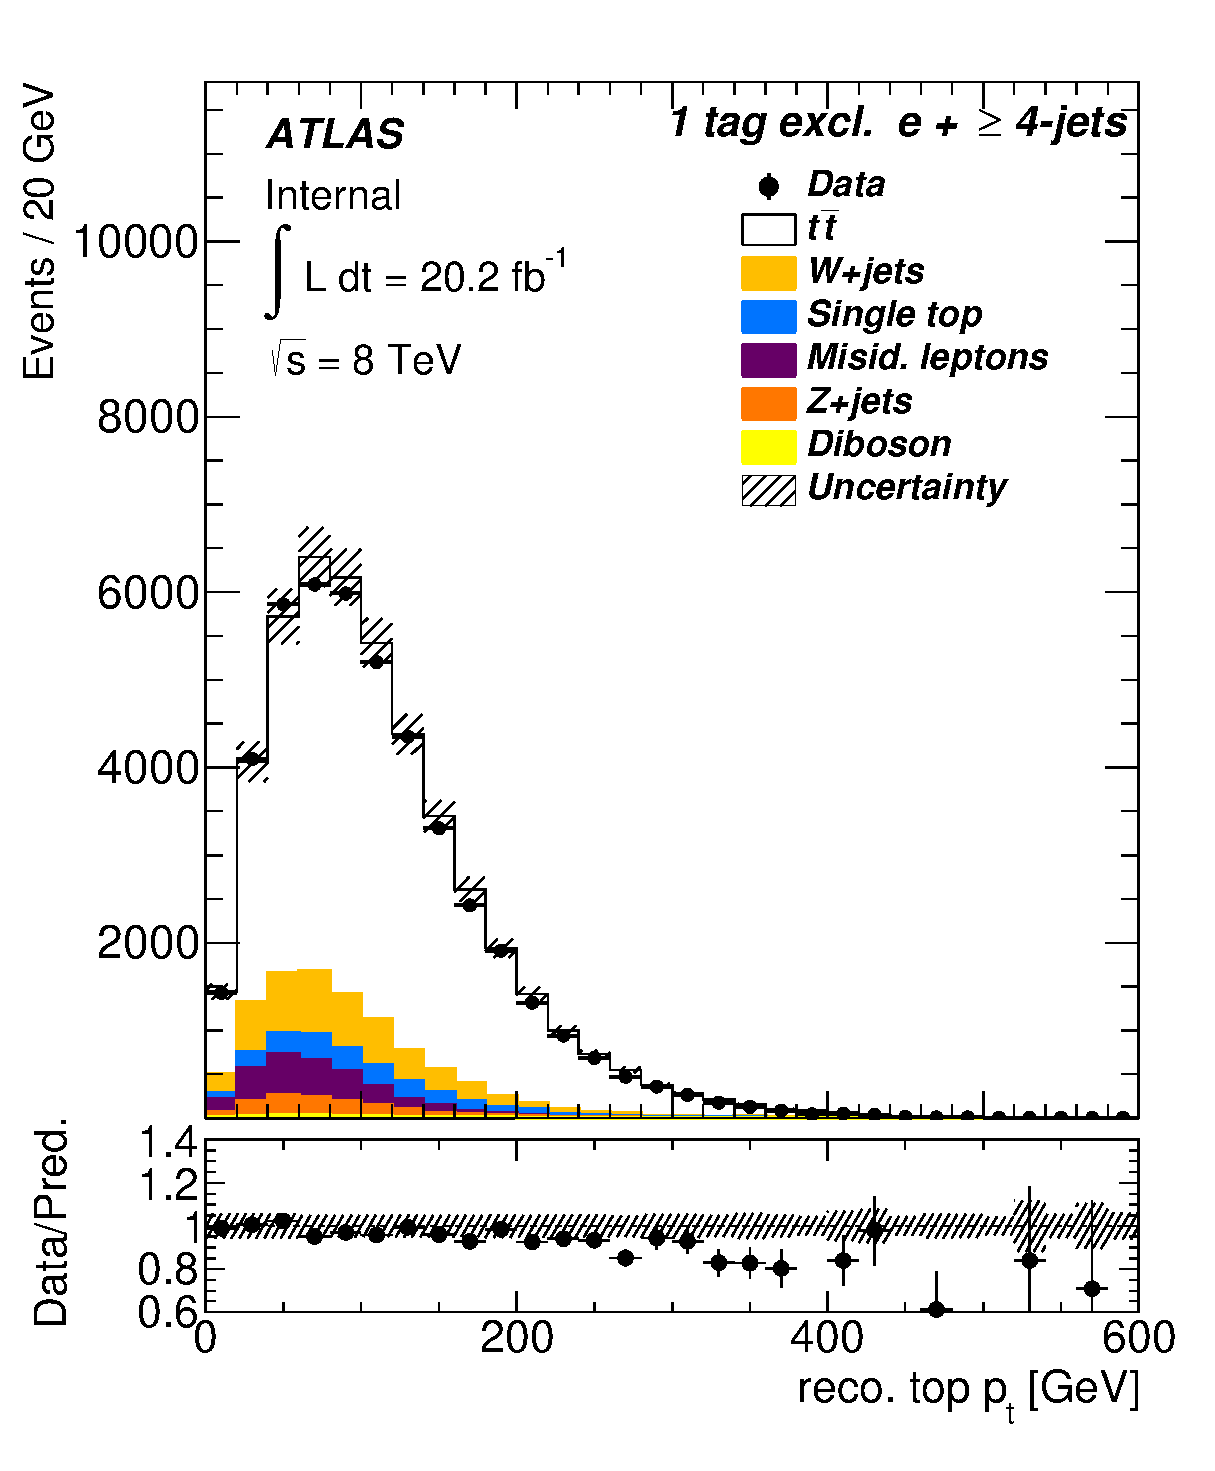
\includegraphics[height=65mm]{chapters/whel/figures/control_Plots2/bTag_1excl/reco_Top_pt_el}
		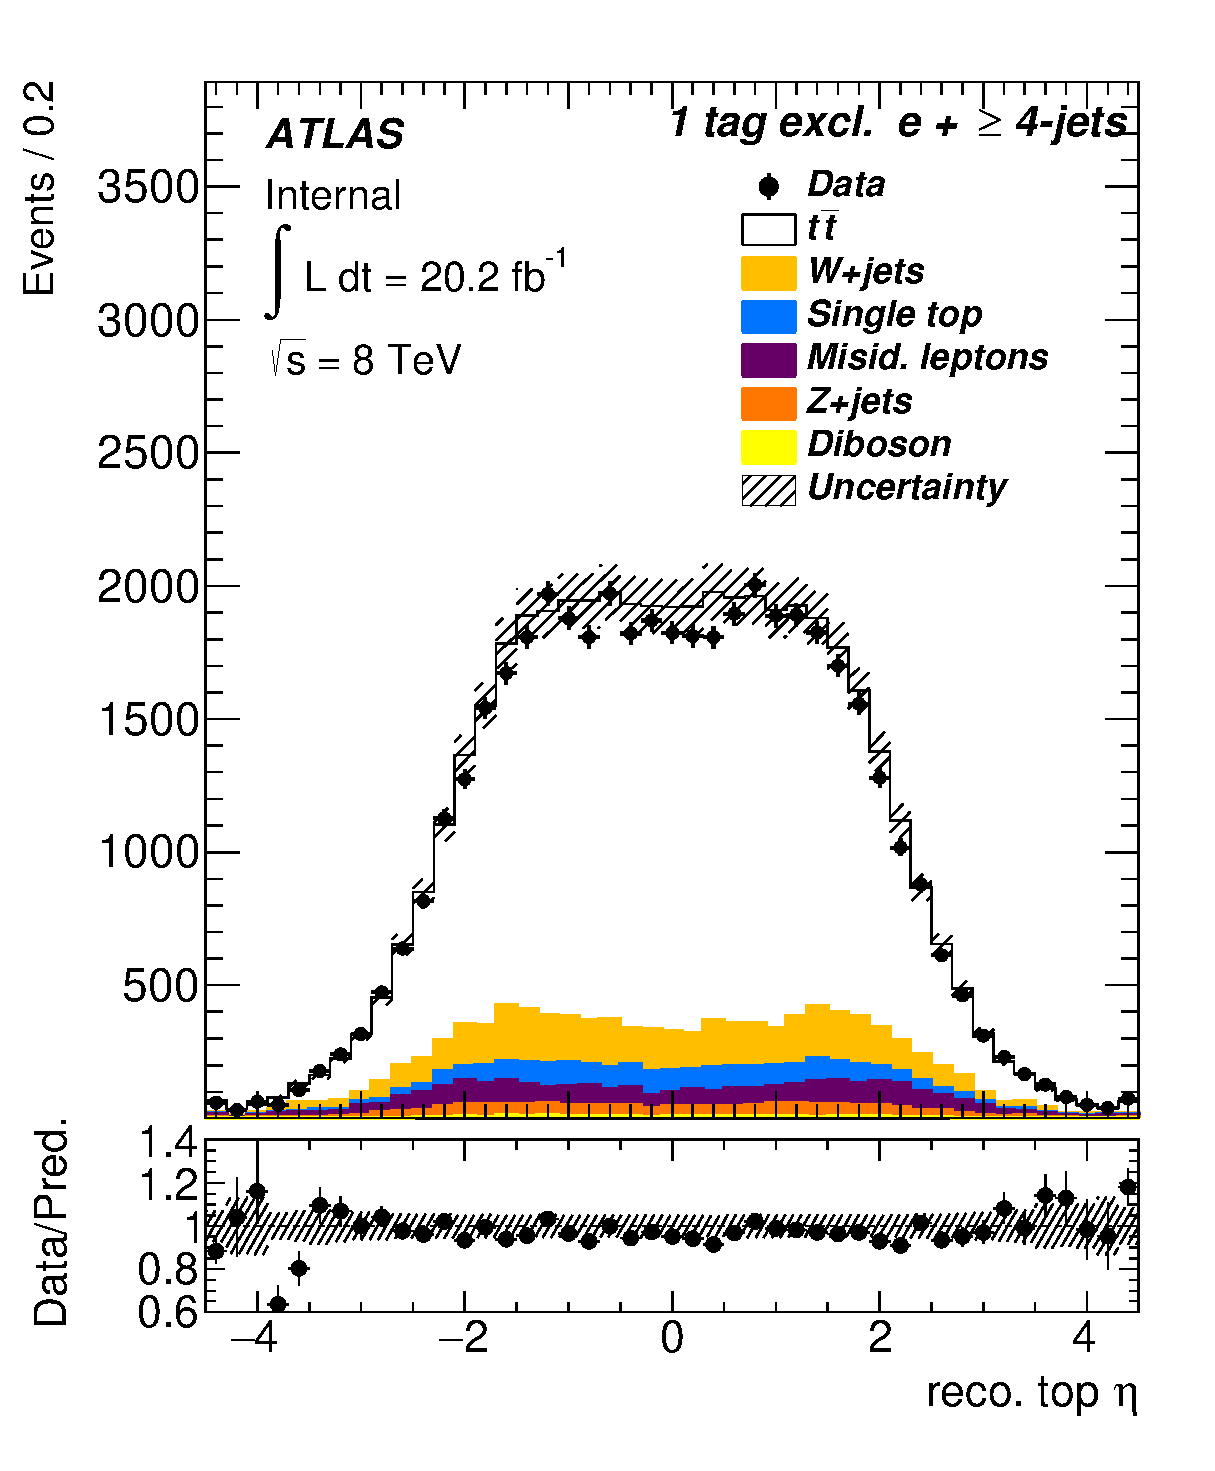
\includegraphics[height=65mm]{chapters/whel/figures/control_Plots2/bTag_1excl/reco_Top_eta_el}\\
		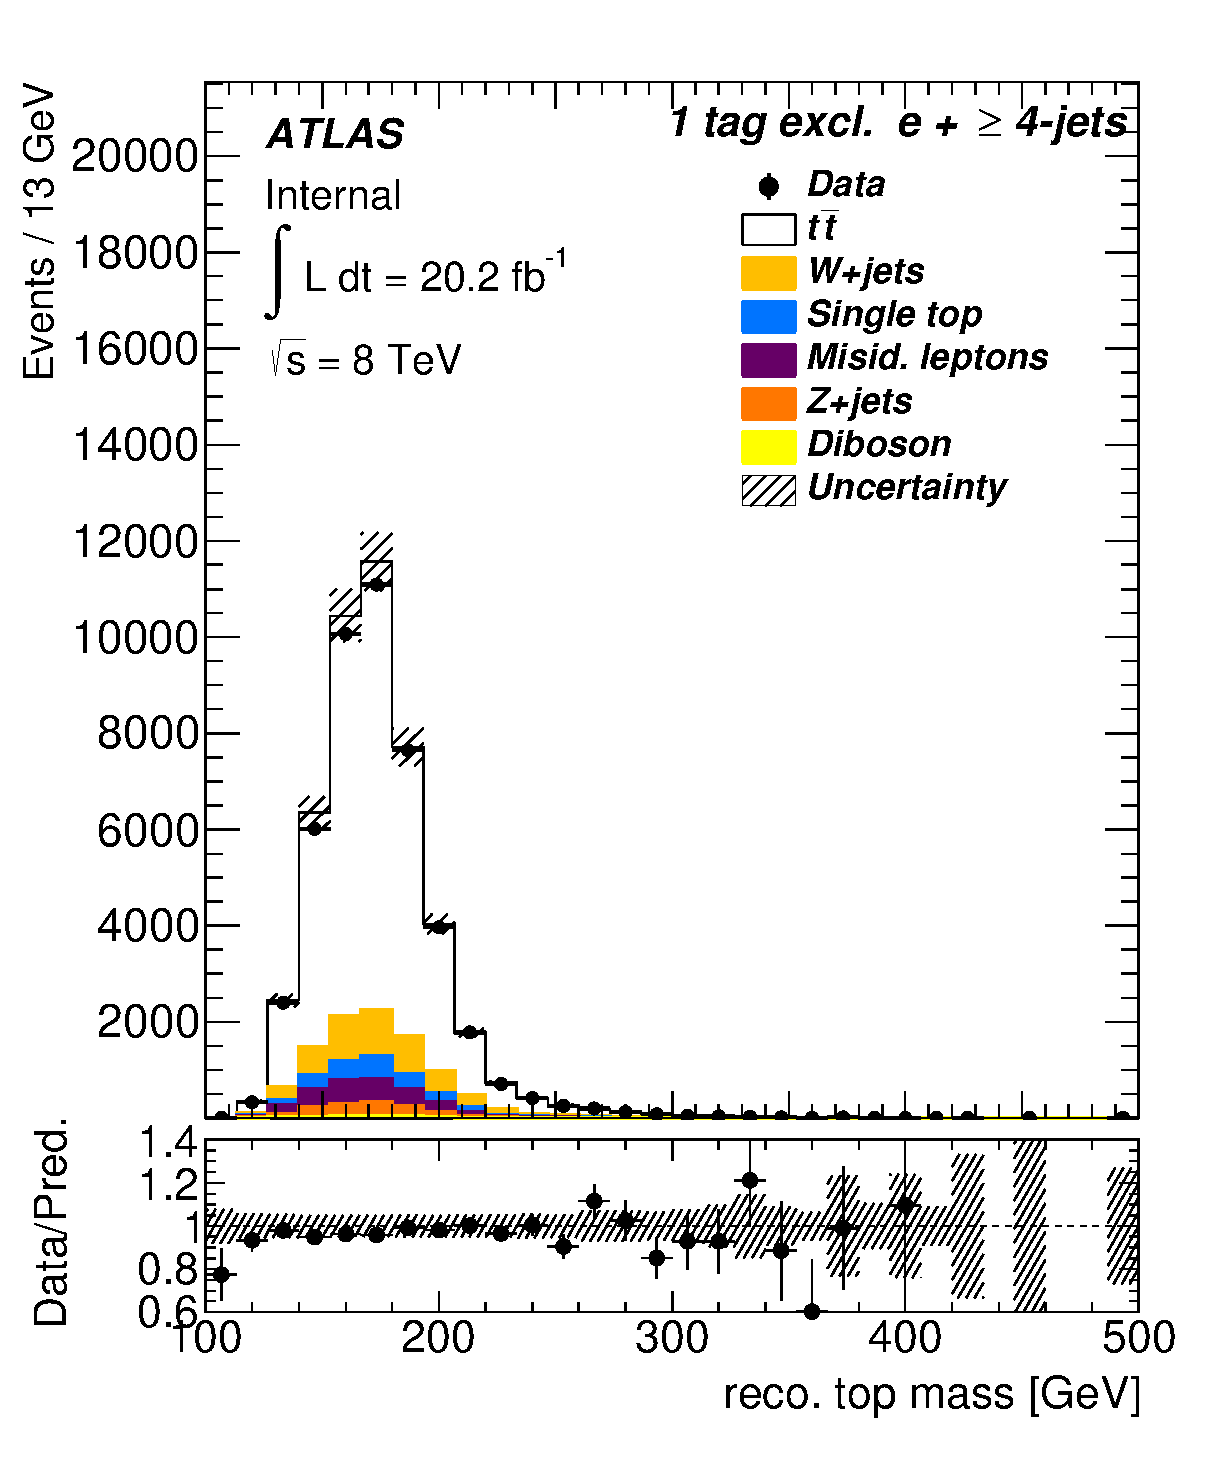
\includegraphics[height=65mm]{chapters/whel/figures/control_Plots2/bTag_1excl/reco_Top_m_el}
		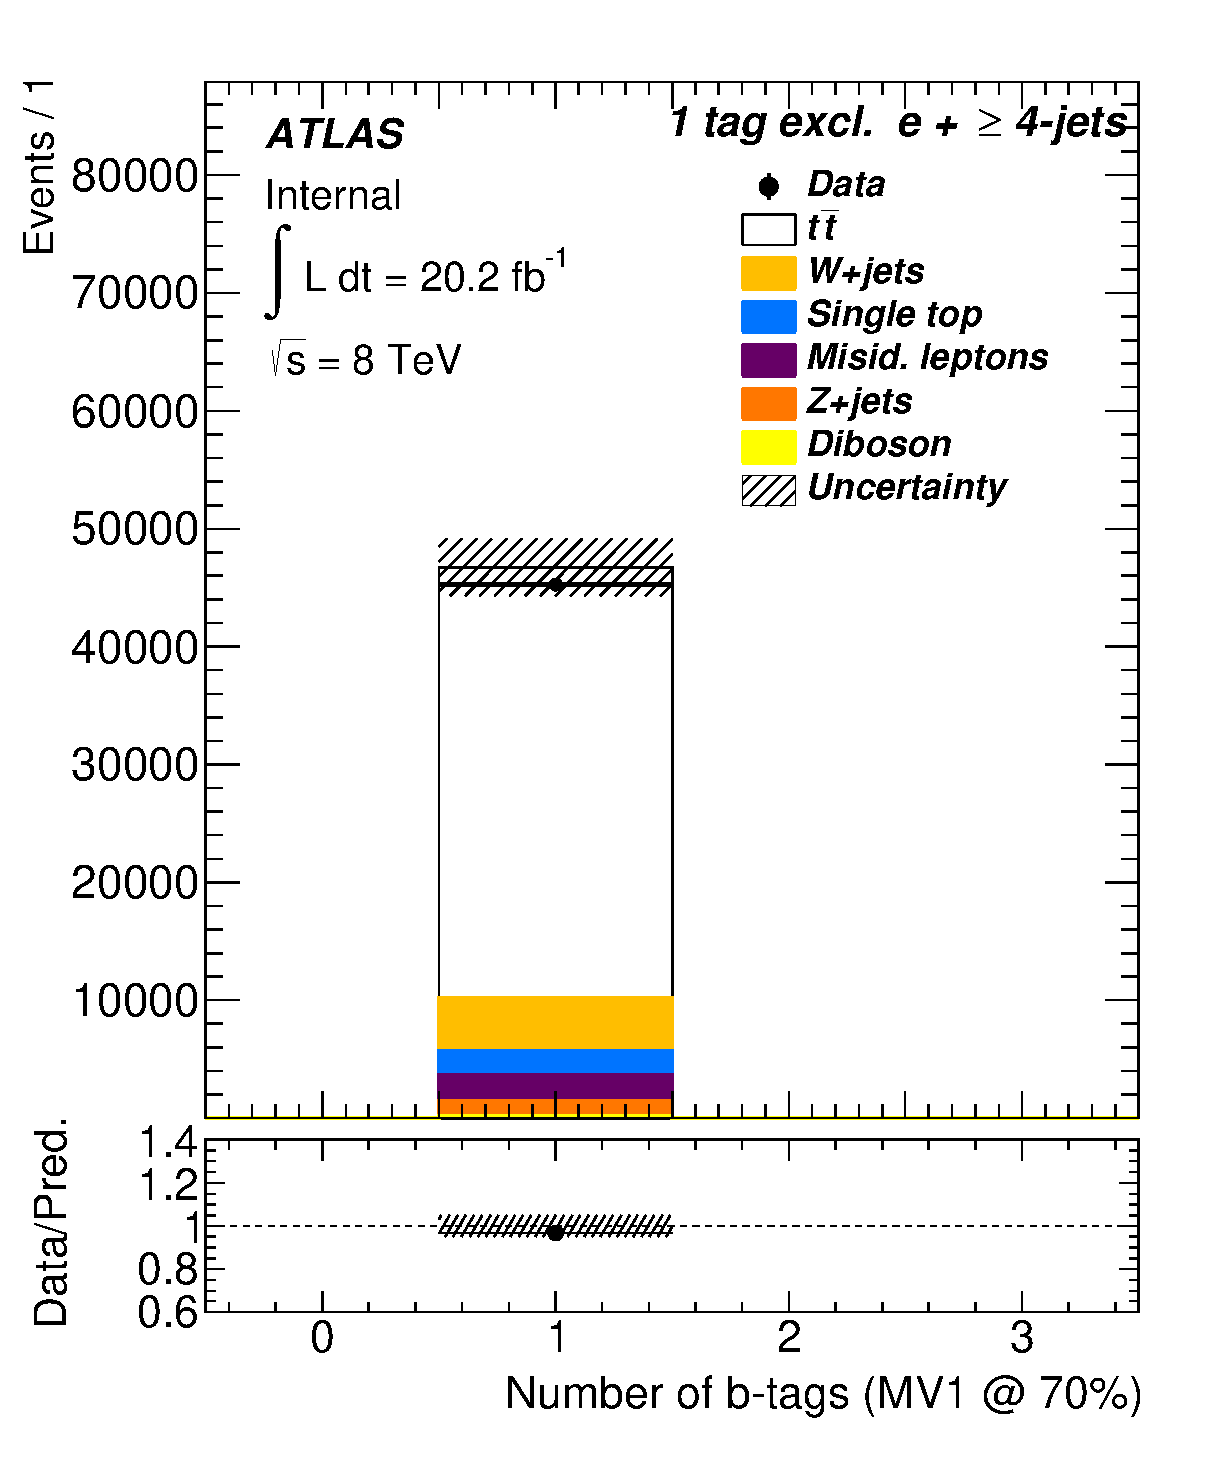
\includegraphics[height=65mm]{chapters/whel/figures/control_Plots2/bTag_1excl/NumberBtags_el}\\
		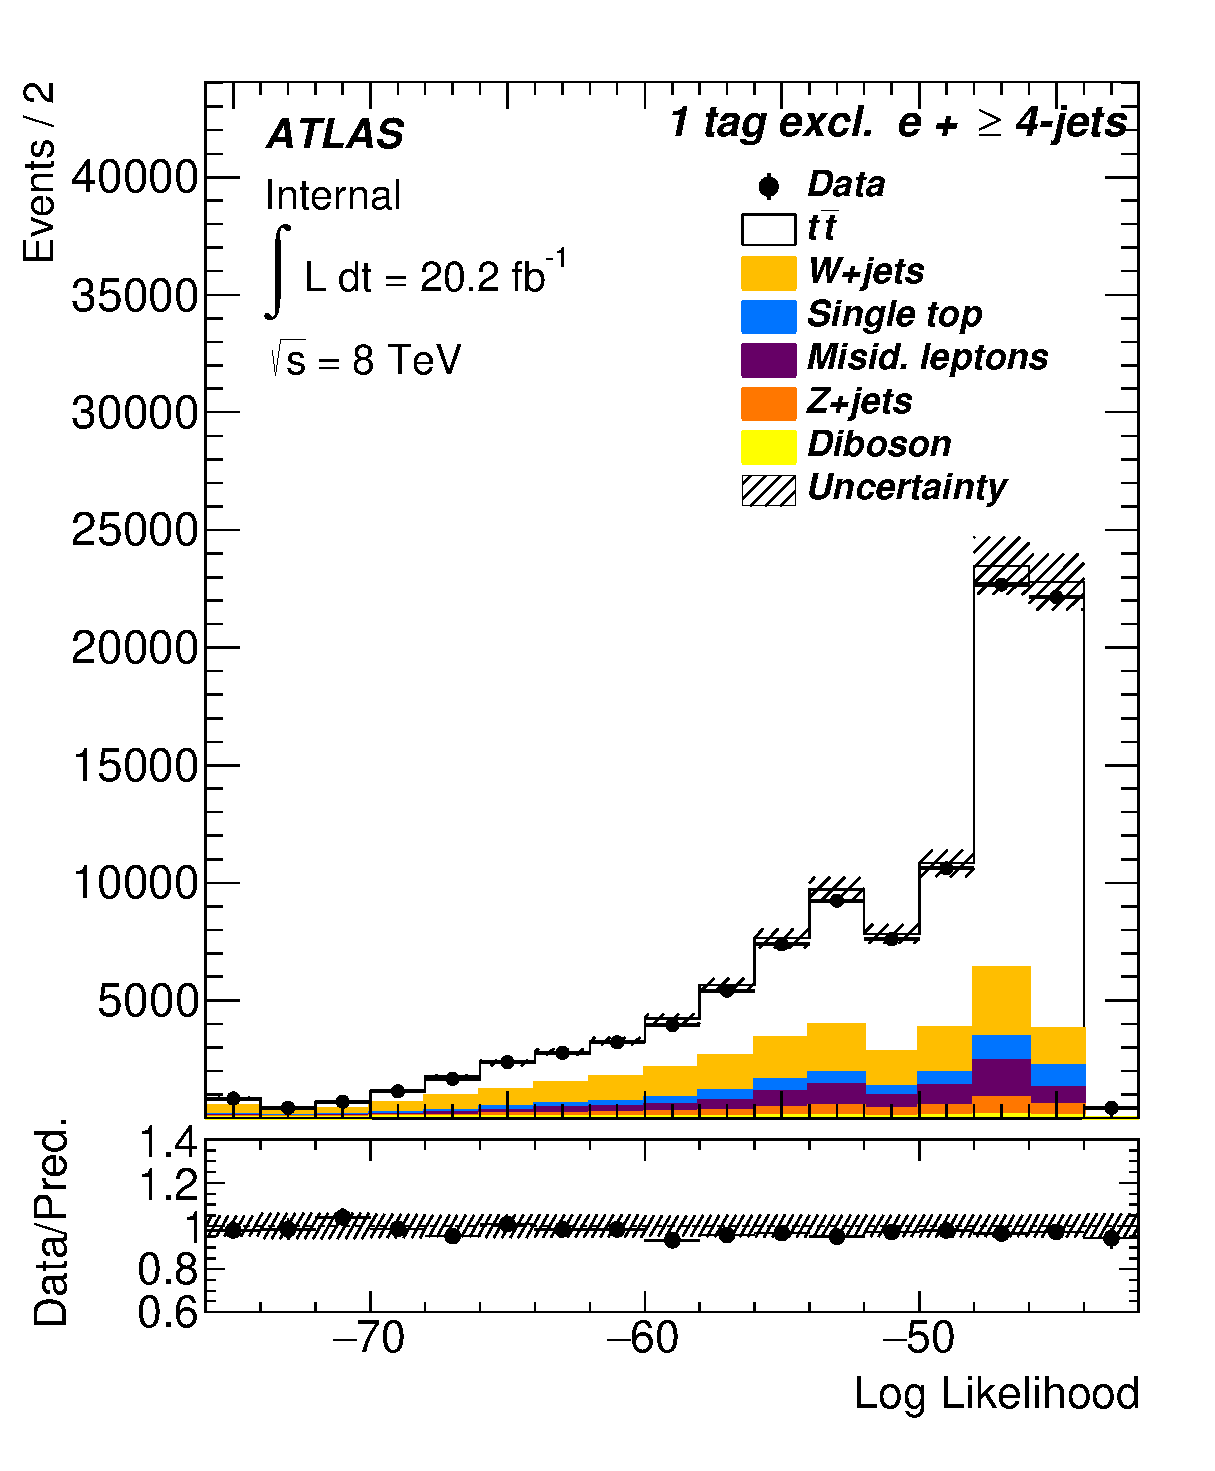
\includegraphics[height=65mm]{chapters/whel/figures/control_Plots2/bTag_1excl_NoLHCut/LogLikelihood_el}
        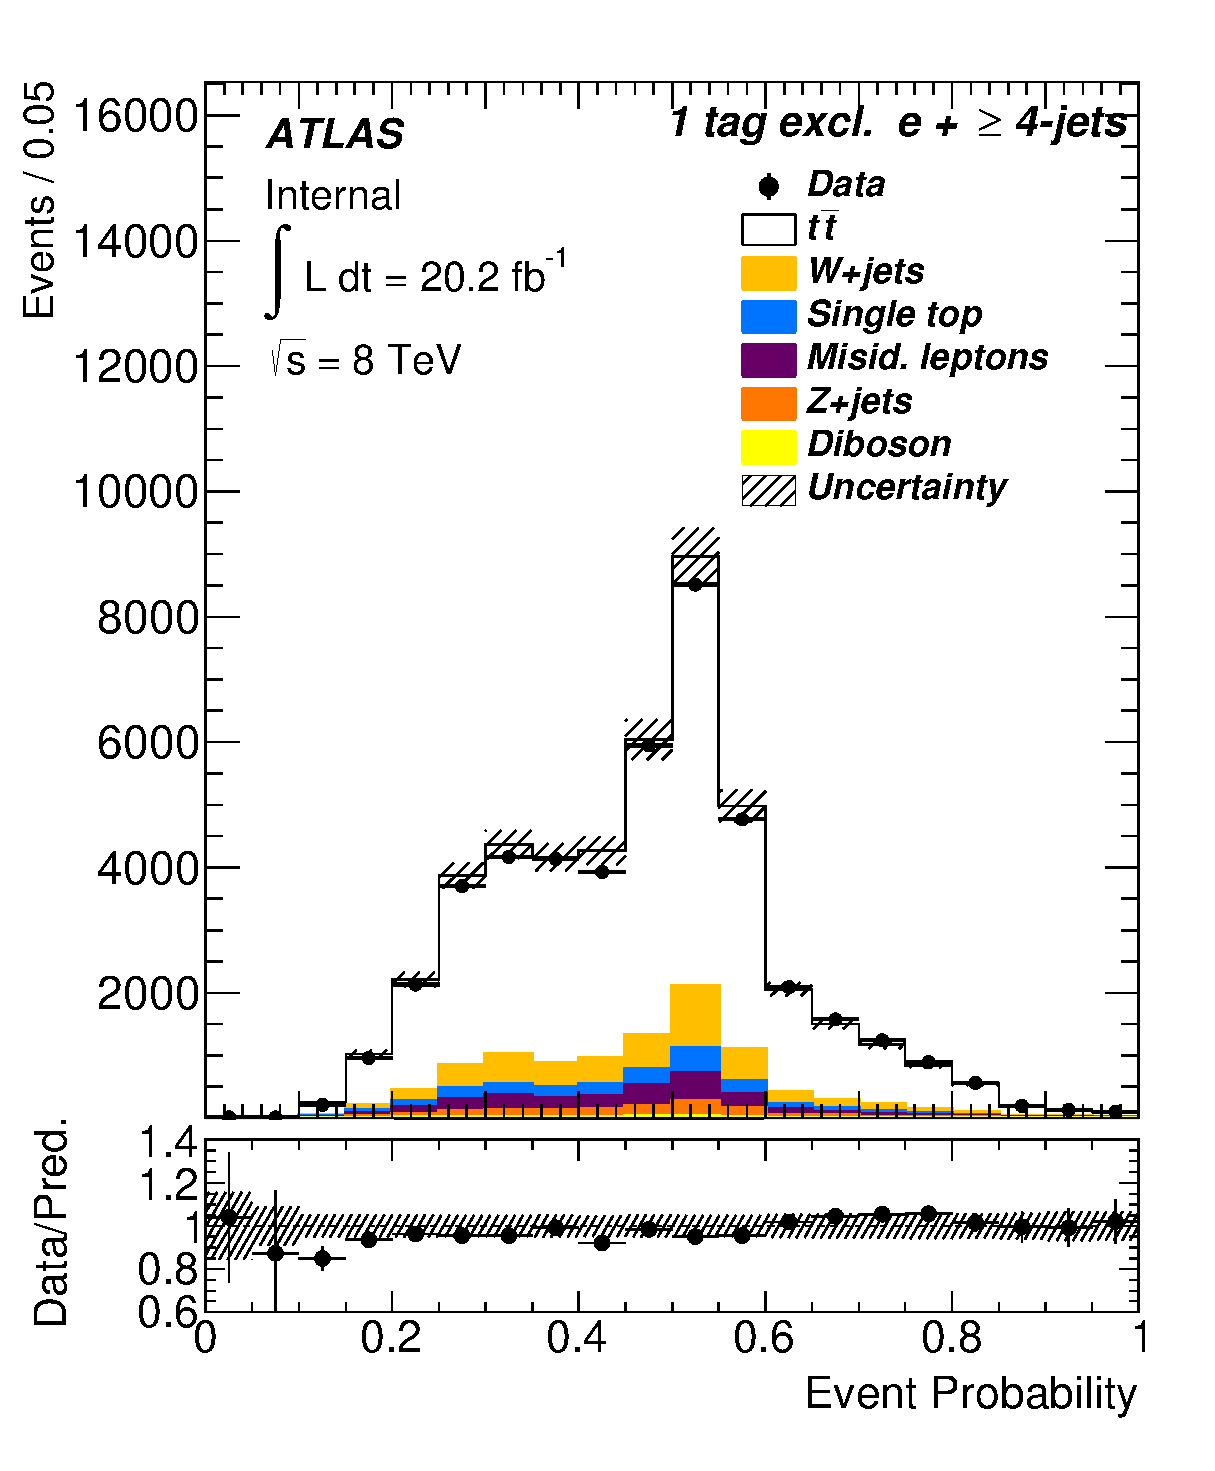
\includegraphics[height=65mm]{chapters/whel/figures/control_Plots2/bTag_1excl/EventProbability_el}
	\caption{Control distributions in the 1 exclusive \bt tag, electron channel for selected top kinematics, the log likelihood, and the event probability distributions of the leading permutation (ranked by event probability). All plots except for the log likelihood are shown after the cut LH $> -48$. The shaded bands represent the Monte Carlo statistical uncertainties.}
	\label{fig:klfitter_control_plots_1}
	\end{center}    
	\end{figure}    
	
\begin{figure}[!h]
\begin{center}
		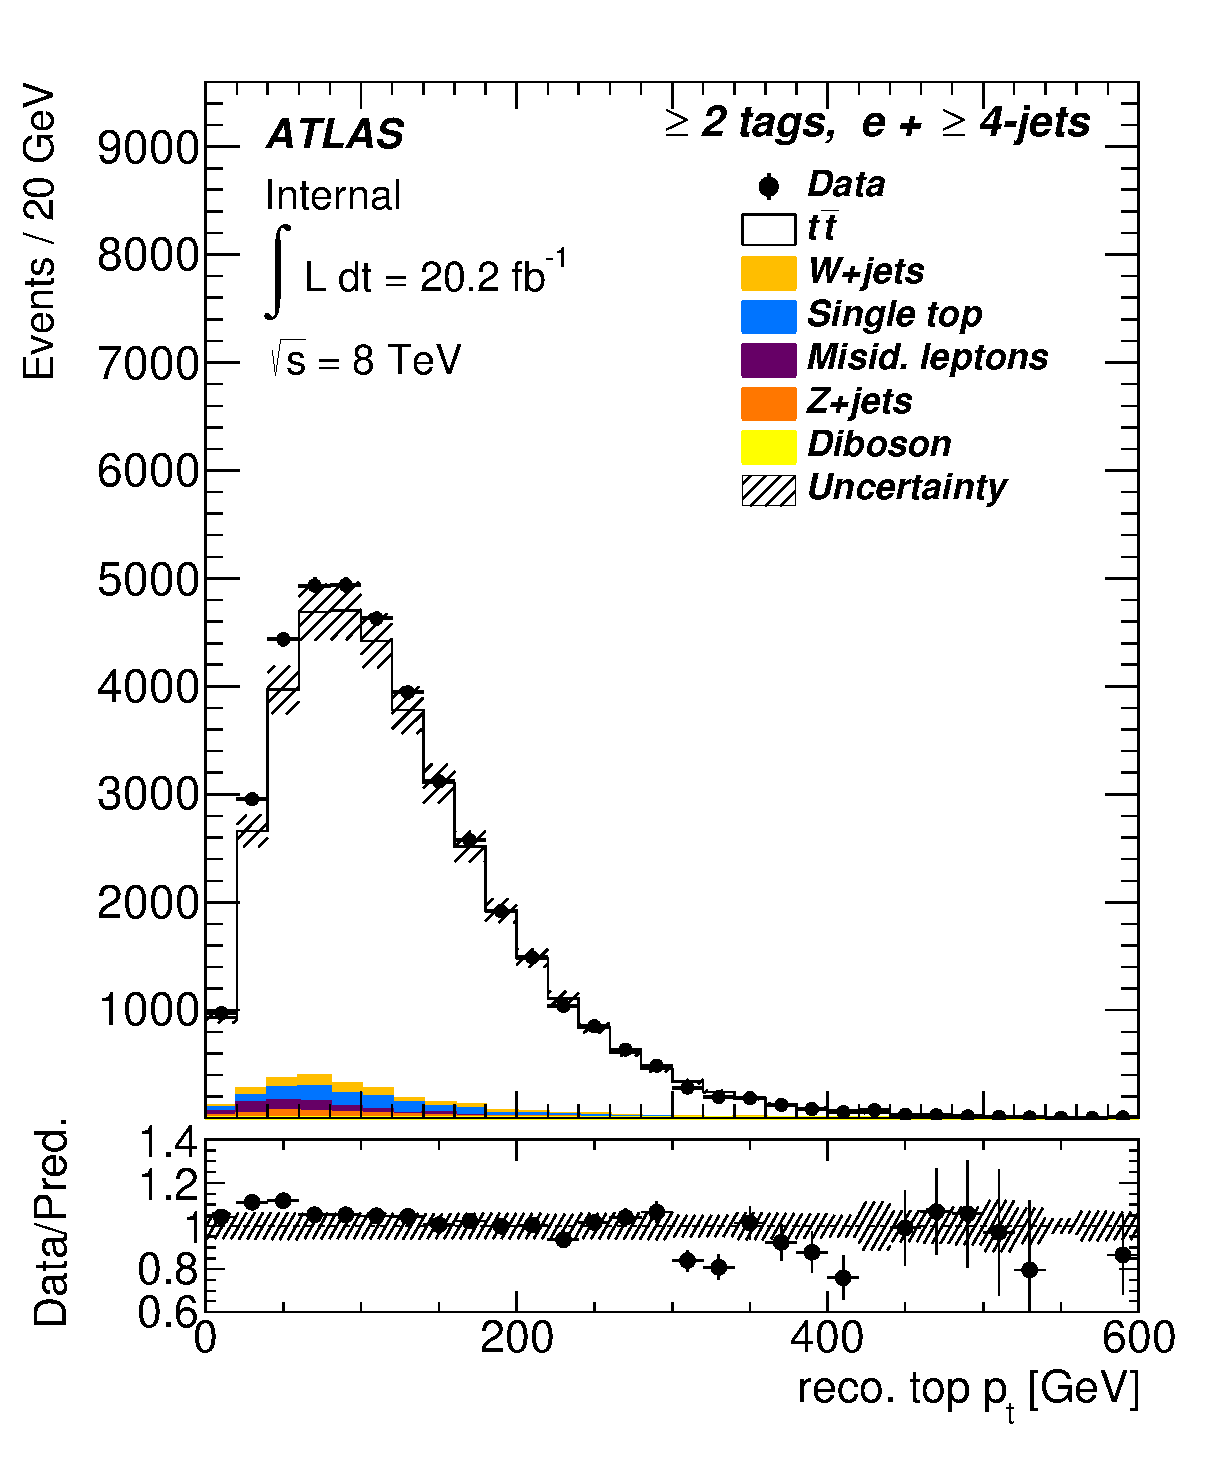
\includegraphics[height=65mm]{chapters/whel/figures/control_Plots2/bTag_2incl/reco_Top_pt_el}
		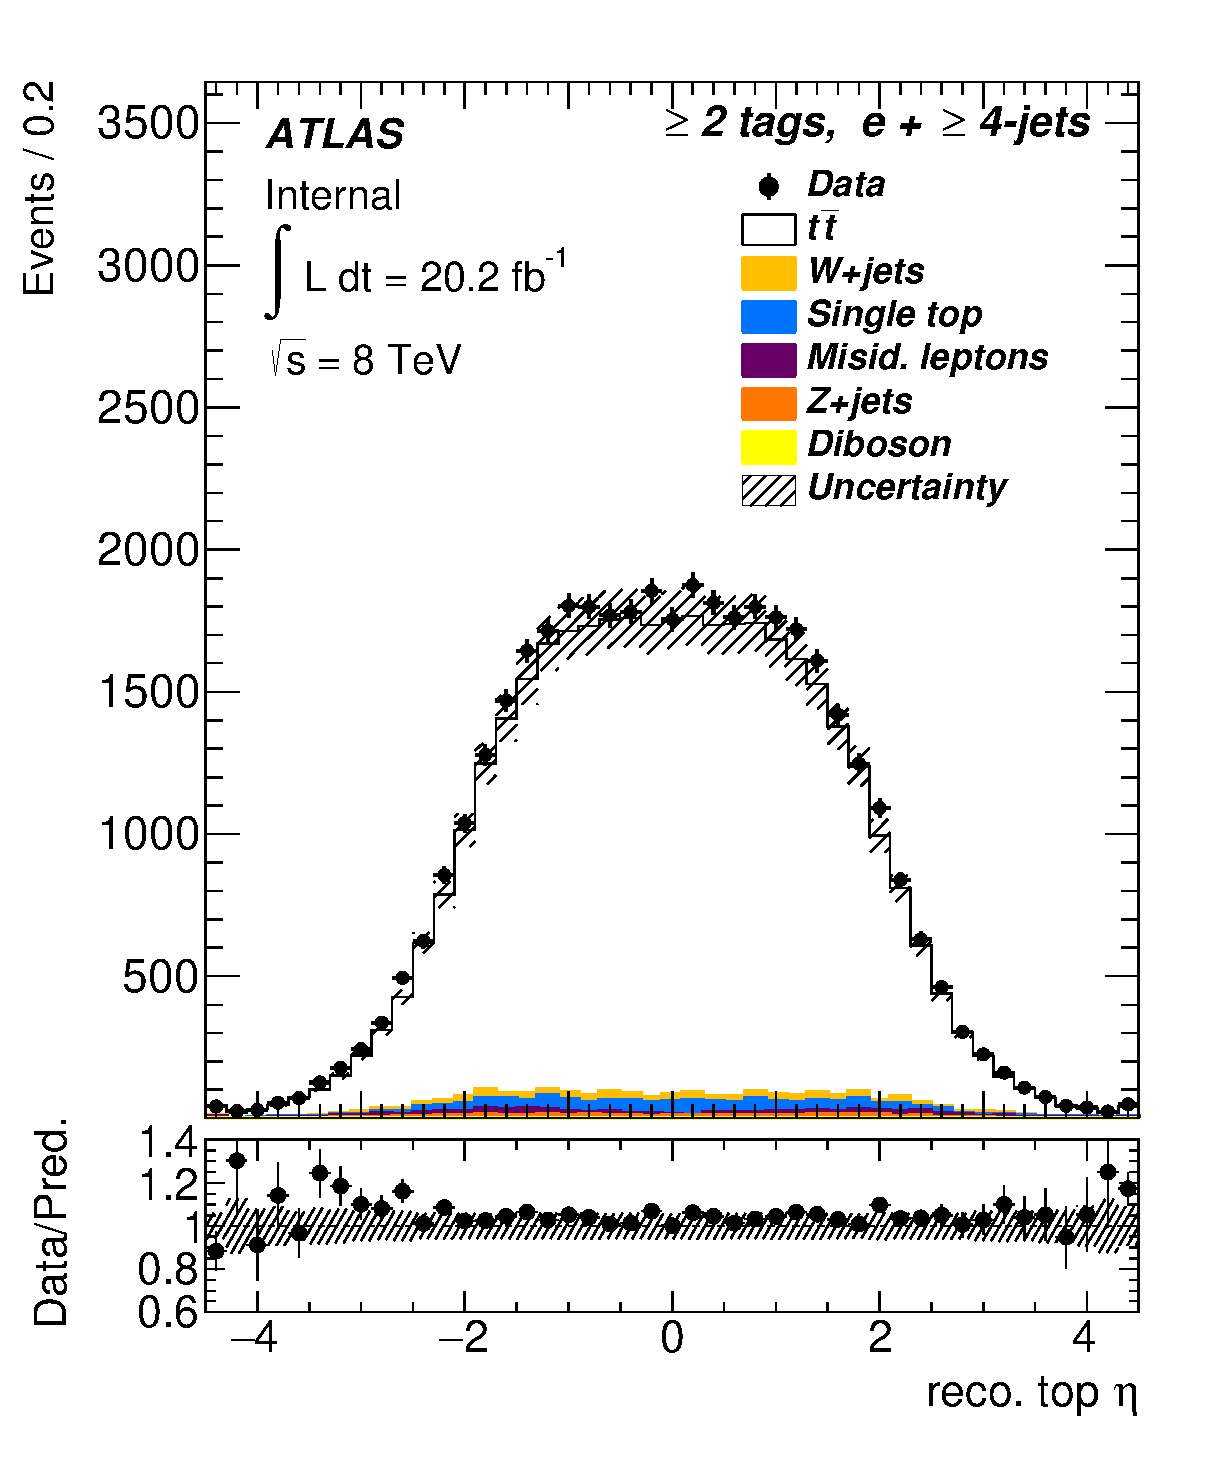
\includegraphics[height=65mm]{chapters/whel/figures/control_Plots2/bTag_2incl/reco_Top_eta_el}\\
		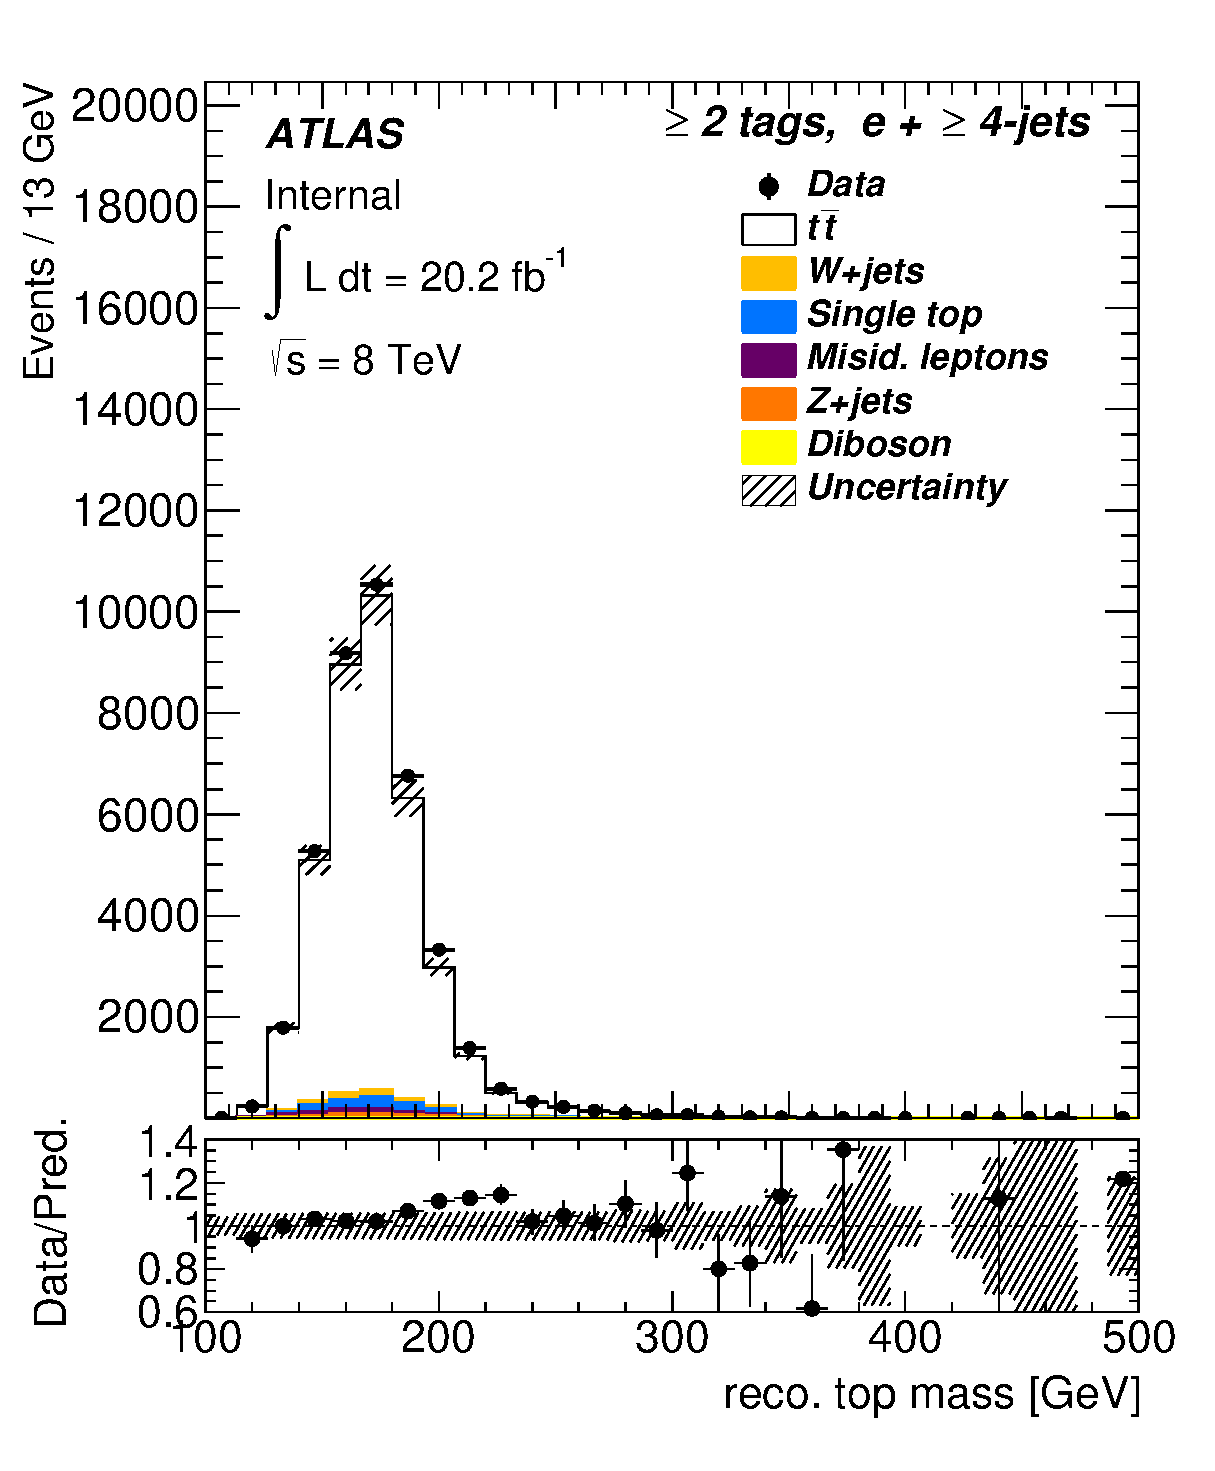
\includegraphics[height=65mm]{chapters/whel/figures/control_Plots2/bTag_2incl/reco_Top_m_el}
		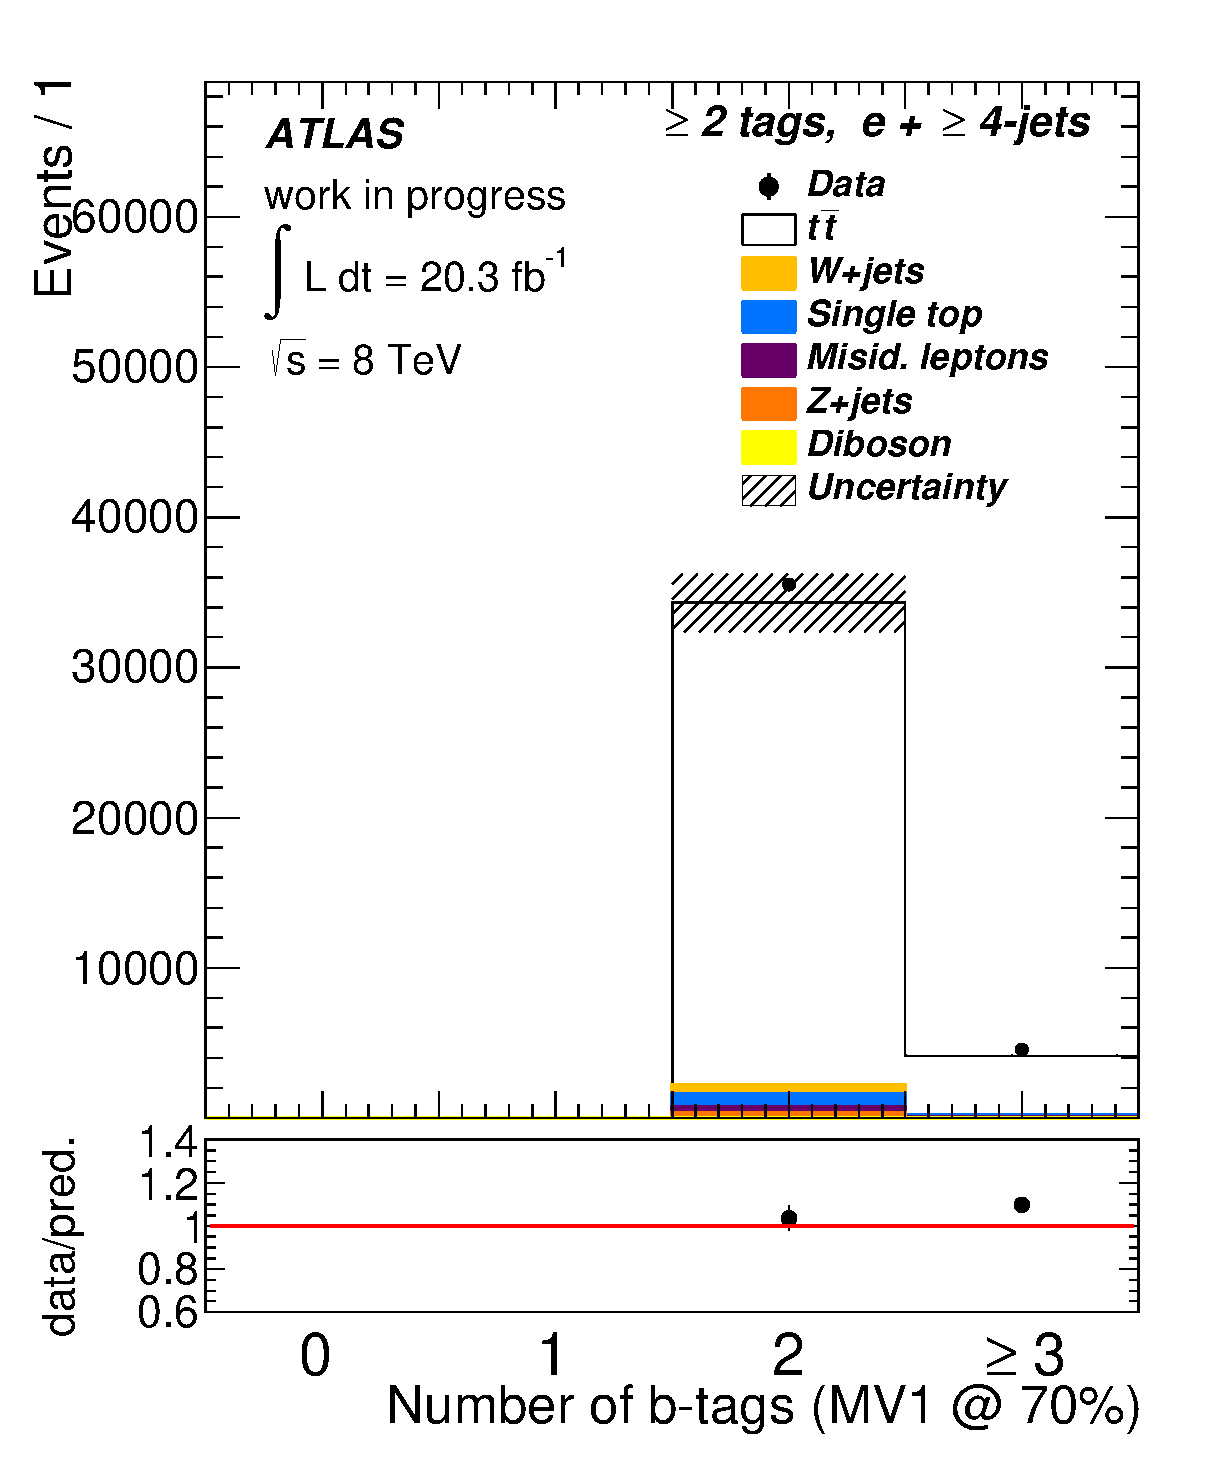
\includegraphics[height=65mm]{chapters/whel/figures/control_Plots2/bTag_2incl/NumberBtags_el}\\
		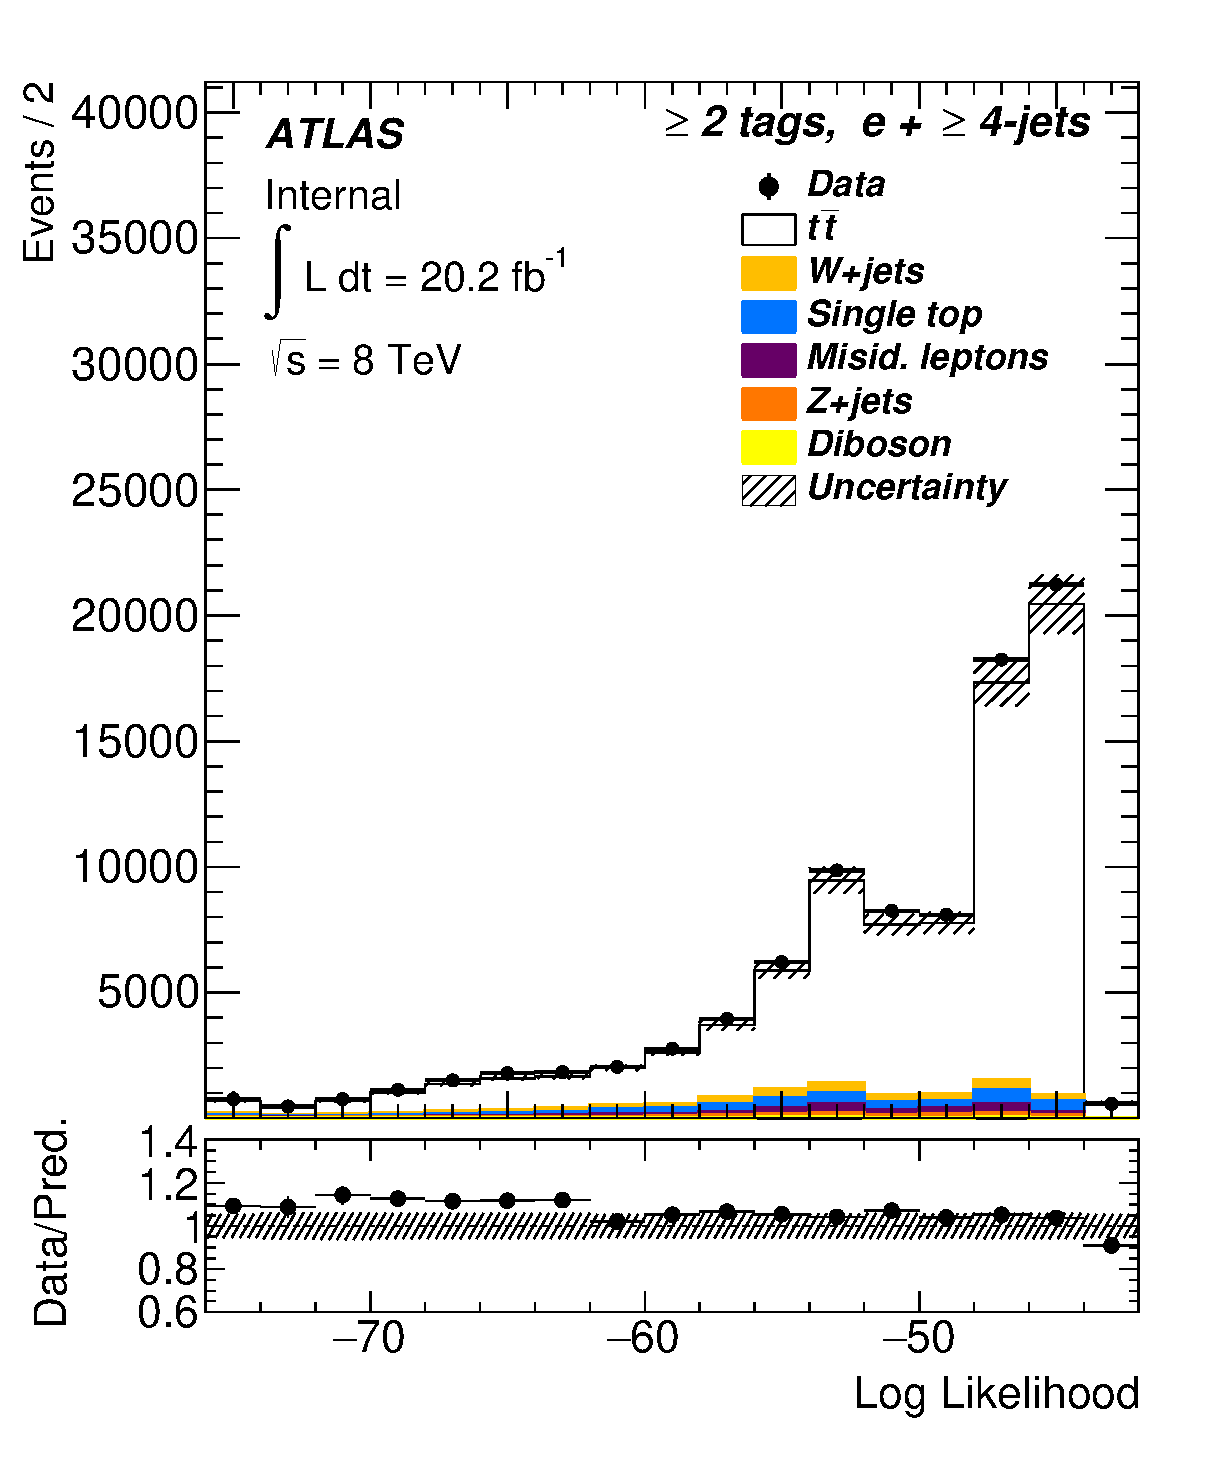
\includegraphics[height=65mm]{chapters/whel/figures/control_Plots2/bTag_2incl_NoLHCut/LogLikelihood_el}
        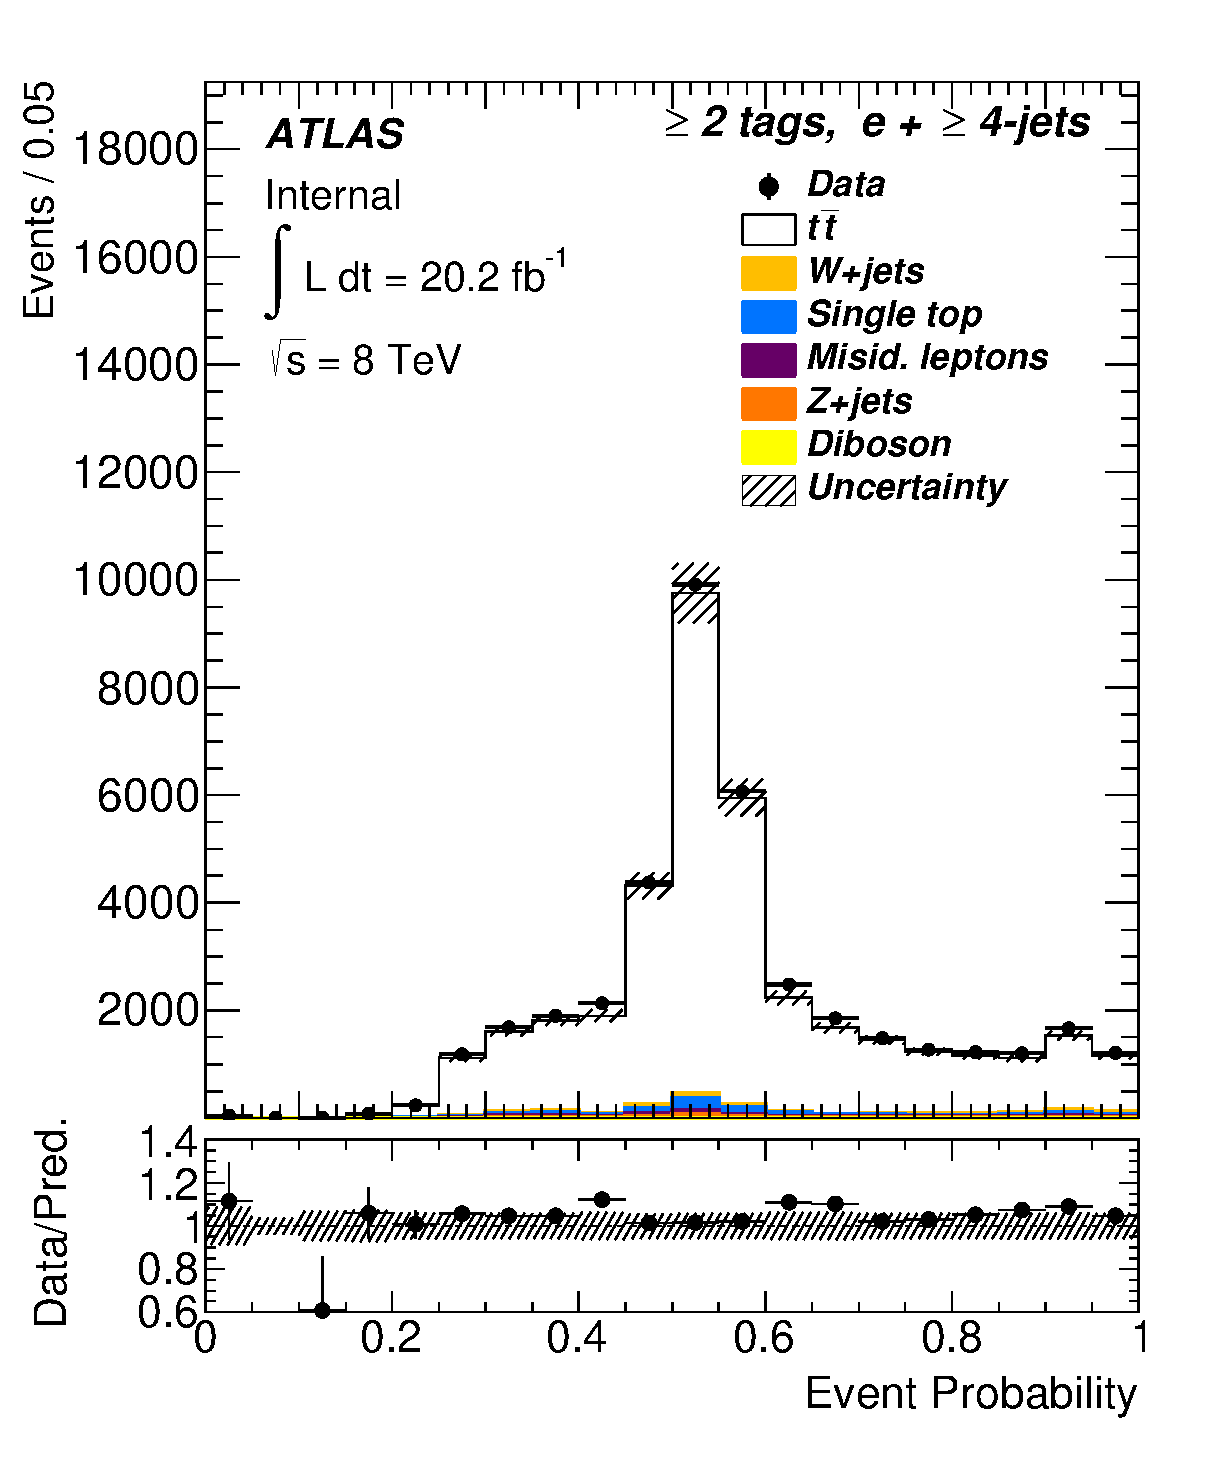
\includegraphics[height=65mm]{chapters/whel/figures/control_Plots2/bTag_2incl/EventProbability_el}
	\caption{Control distributions in the 2 inclusive \bt tag, electron channel for selected top kinematics, the log likelihood, and the event probability distributions of the leading permutation (ranked by event probability). All plots except for the log likelihood are shown after the cut LH $> -48$. The shaded bands represent the Monte Carlo statistical uncertainties.}
	\label{fig:klfitter_control_plots_2}
	\end{center}    
	\end{figure}
	
\begin{figure}[!h]
\begin{center}
		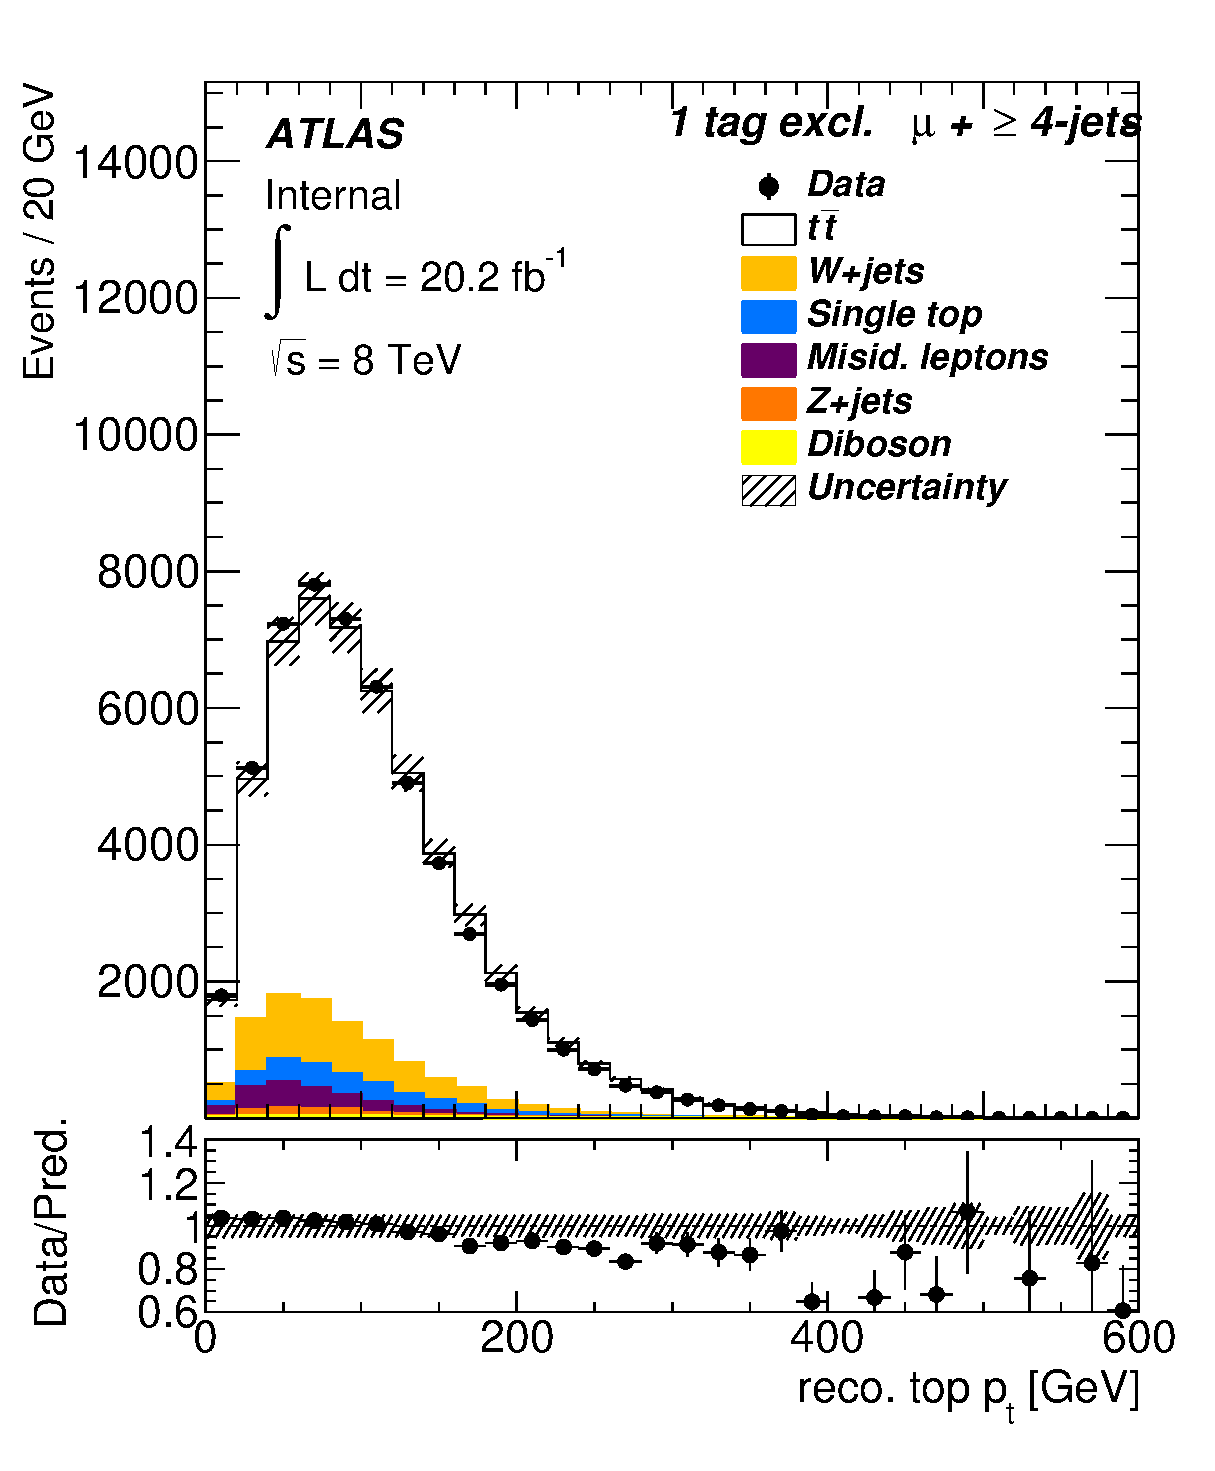
\includegraphics[height=65mm]{chapters/whel/figures/control_Plots2/bTag_1excl/reco_Top_pt_mu}
		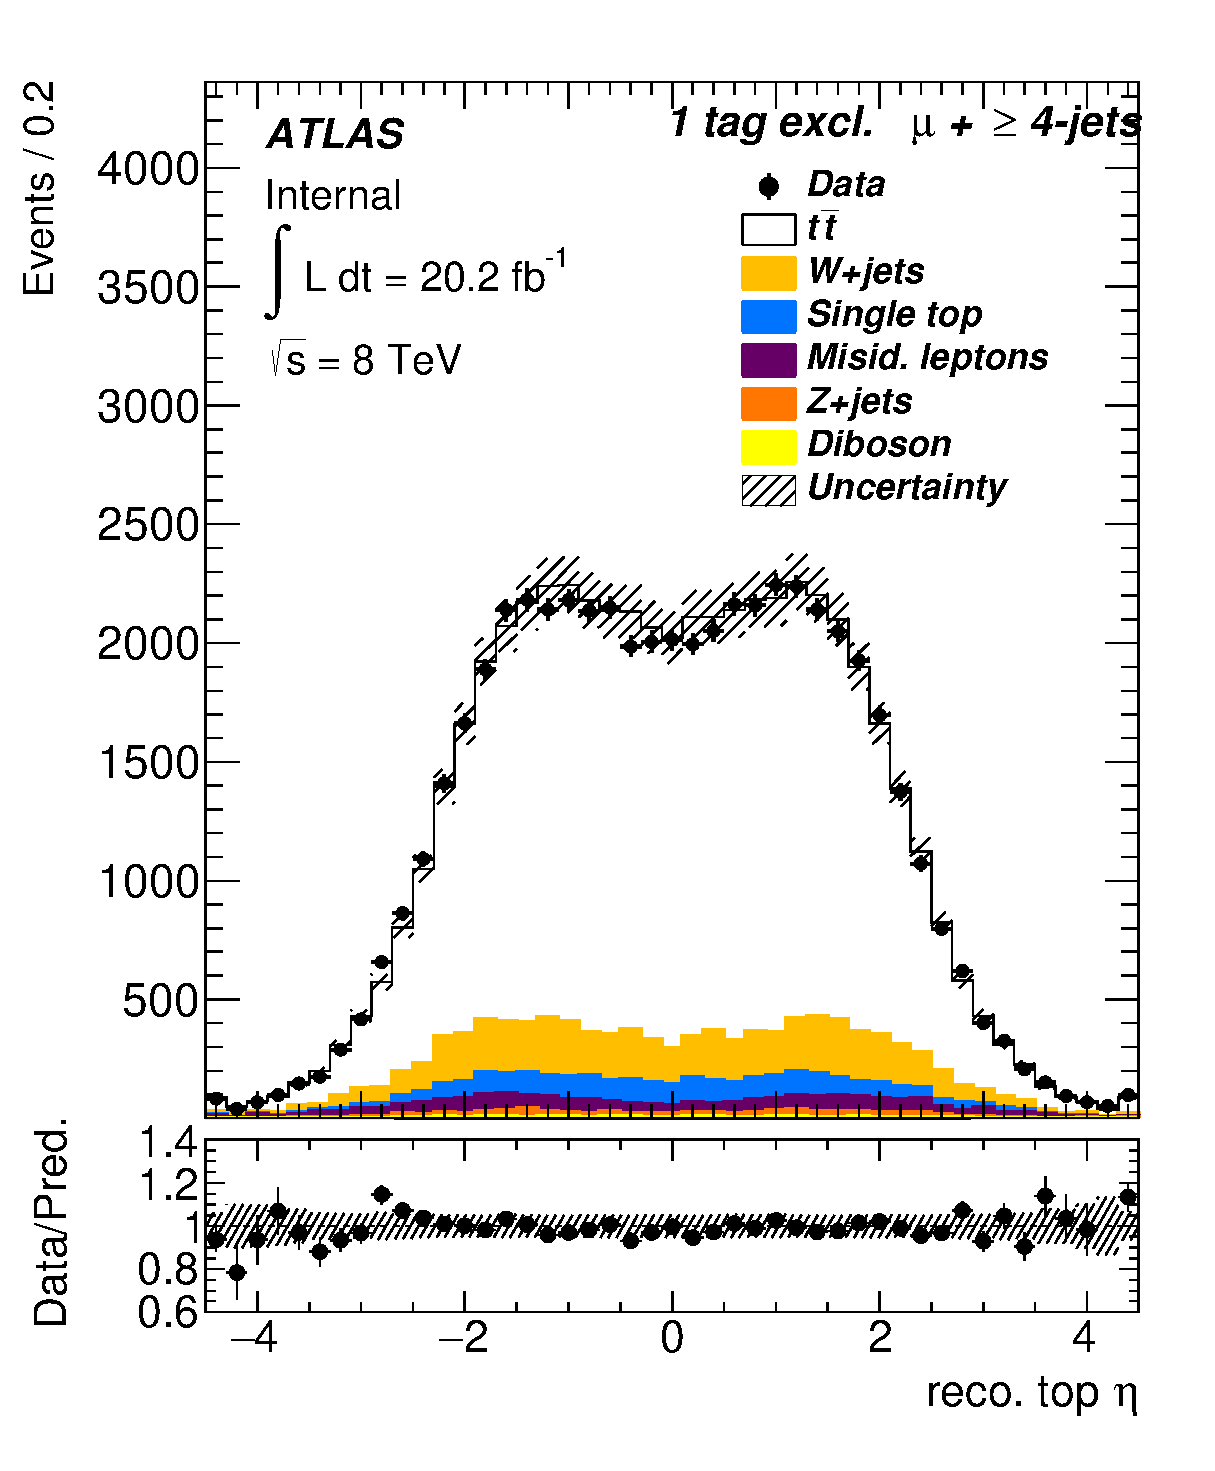
\includegraphics[height=65mm]{chapters/whel/figures/control_Plots2/bTag_1excl/reco_Top_eta_mu}\\
		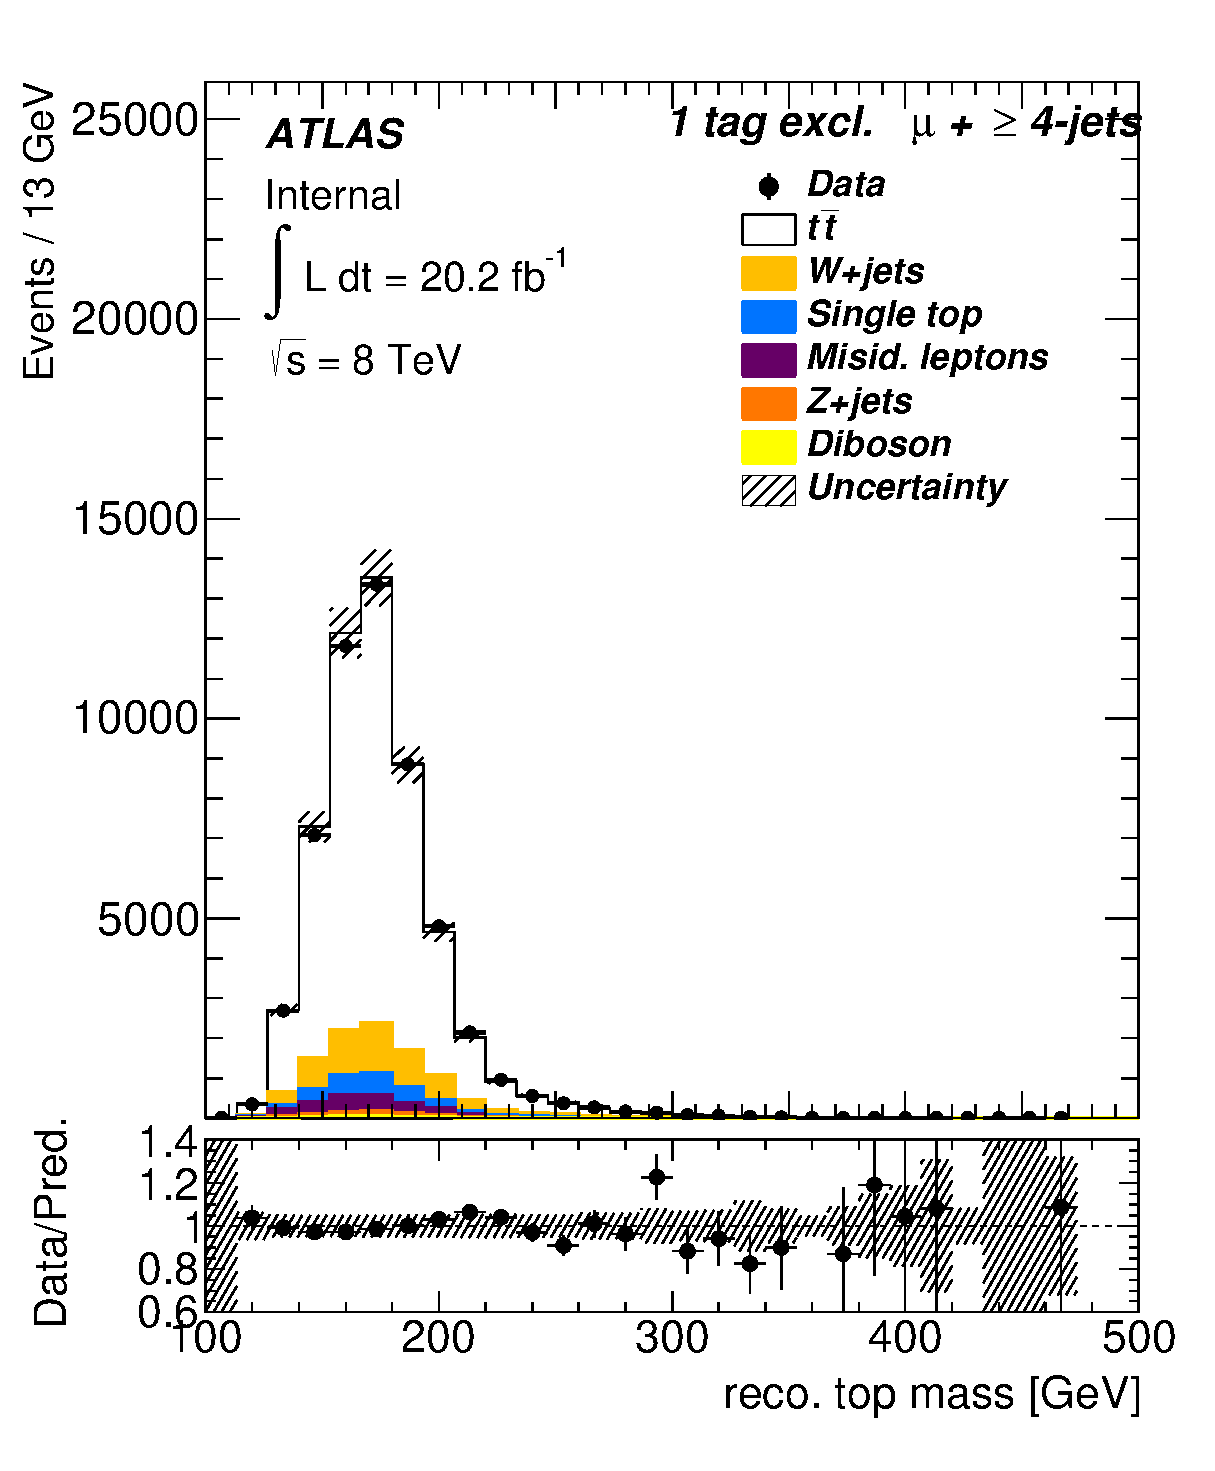
\includegraphics[height=65mm]{chapters/whel/figures/control_Plots2/bTag_1excl/reco_Top_m_mu}
		\includegraphics[height=65mm]{chapters/whel/figures/control_Plots2/bTag_1excl/NumberBtags_mu}\\
		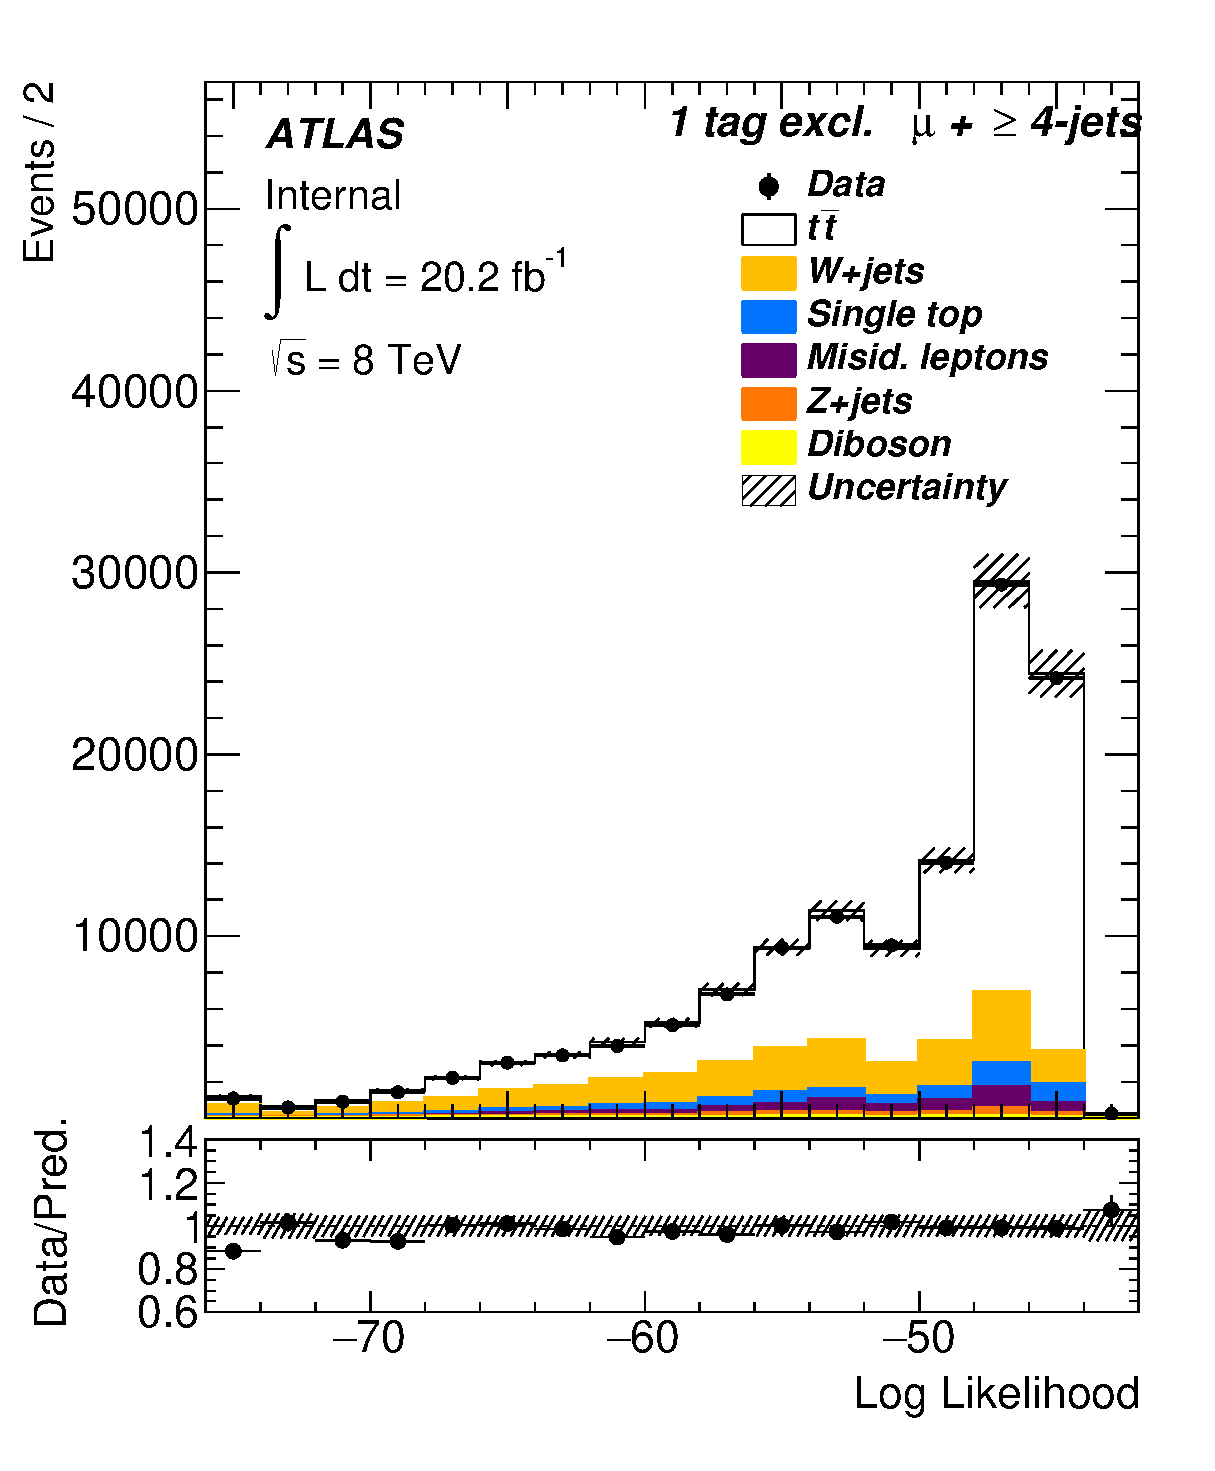
\includegraphics[height=65mm]{chapters/whel/figures/control_Plots2/bTag_1excl_NoLHCut/LogLikelihood_mu}
        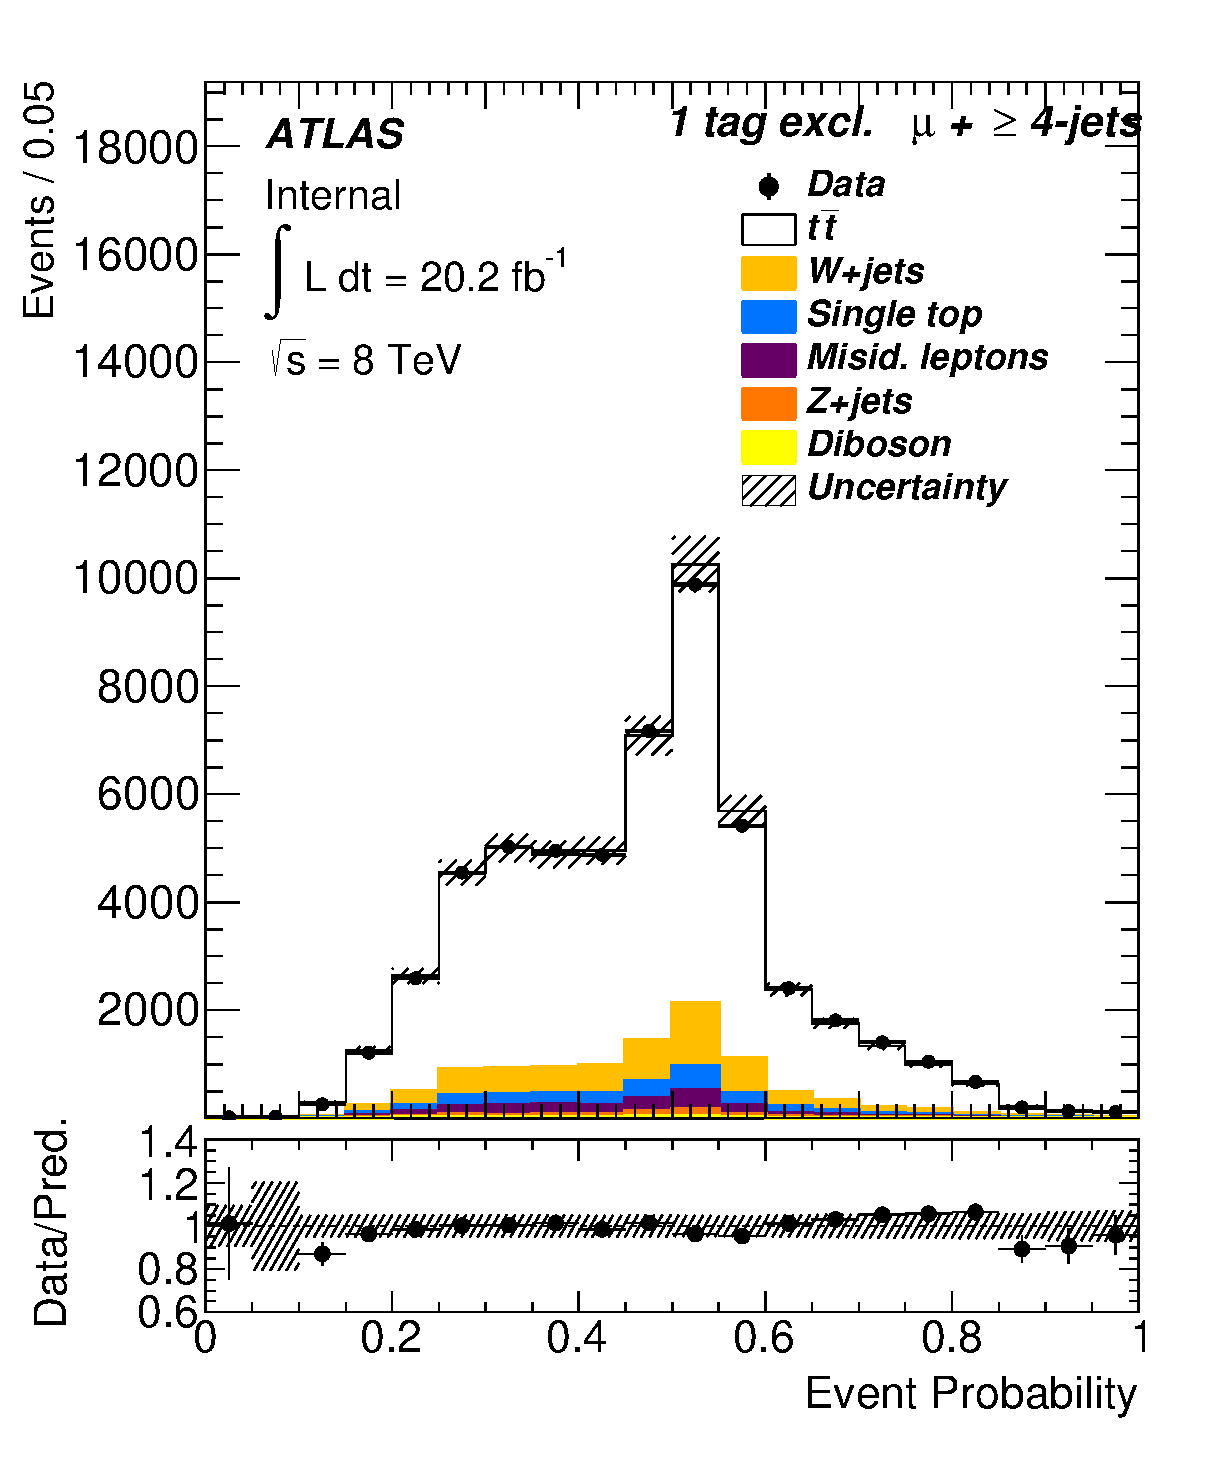
\includegraphics[height=65mm]{chapters/whel/figures/control_Plots2/bTag_1excl/EventProbability_mu}
	\caption{Control distributions in the 1 exclusive \bt tag, muon channel for selected top kinematics, the log likelihood, and the event probability distributions of the leading permutation (ranked by event probability). All plots except for the log likelihood are shown after the cut LH $> -48$. The shaded bands represent the Monte Carlo statistical uncertainties.}
	\label{fig:klfitter_control_plots_3}
	\end{center}    
	\end{figure}    
	
\begin{figure}[!h]
\begin{center}
		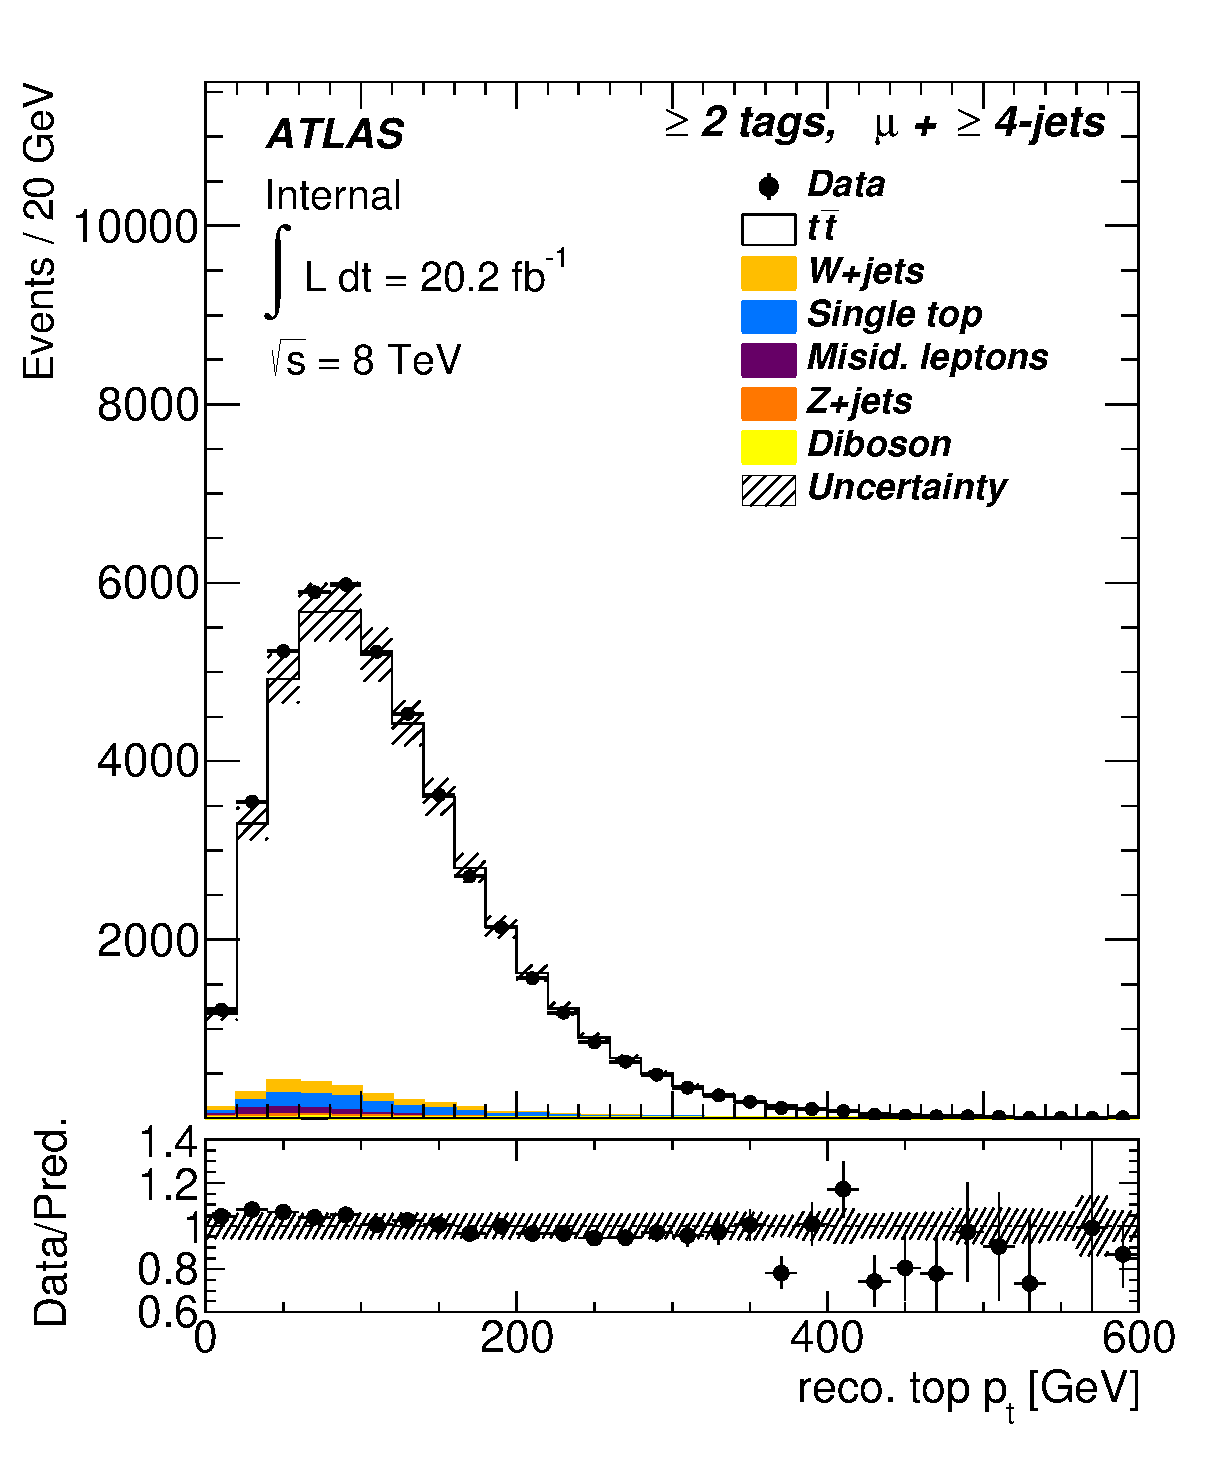
\includegraphics[height=65mm]{chapters/whel/figures/control_Plots2/bTag_2incl/reco_Top_pt_mu}
		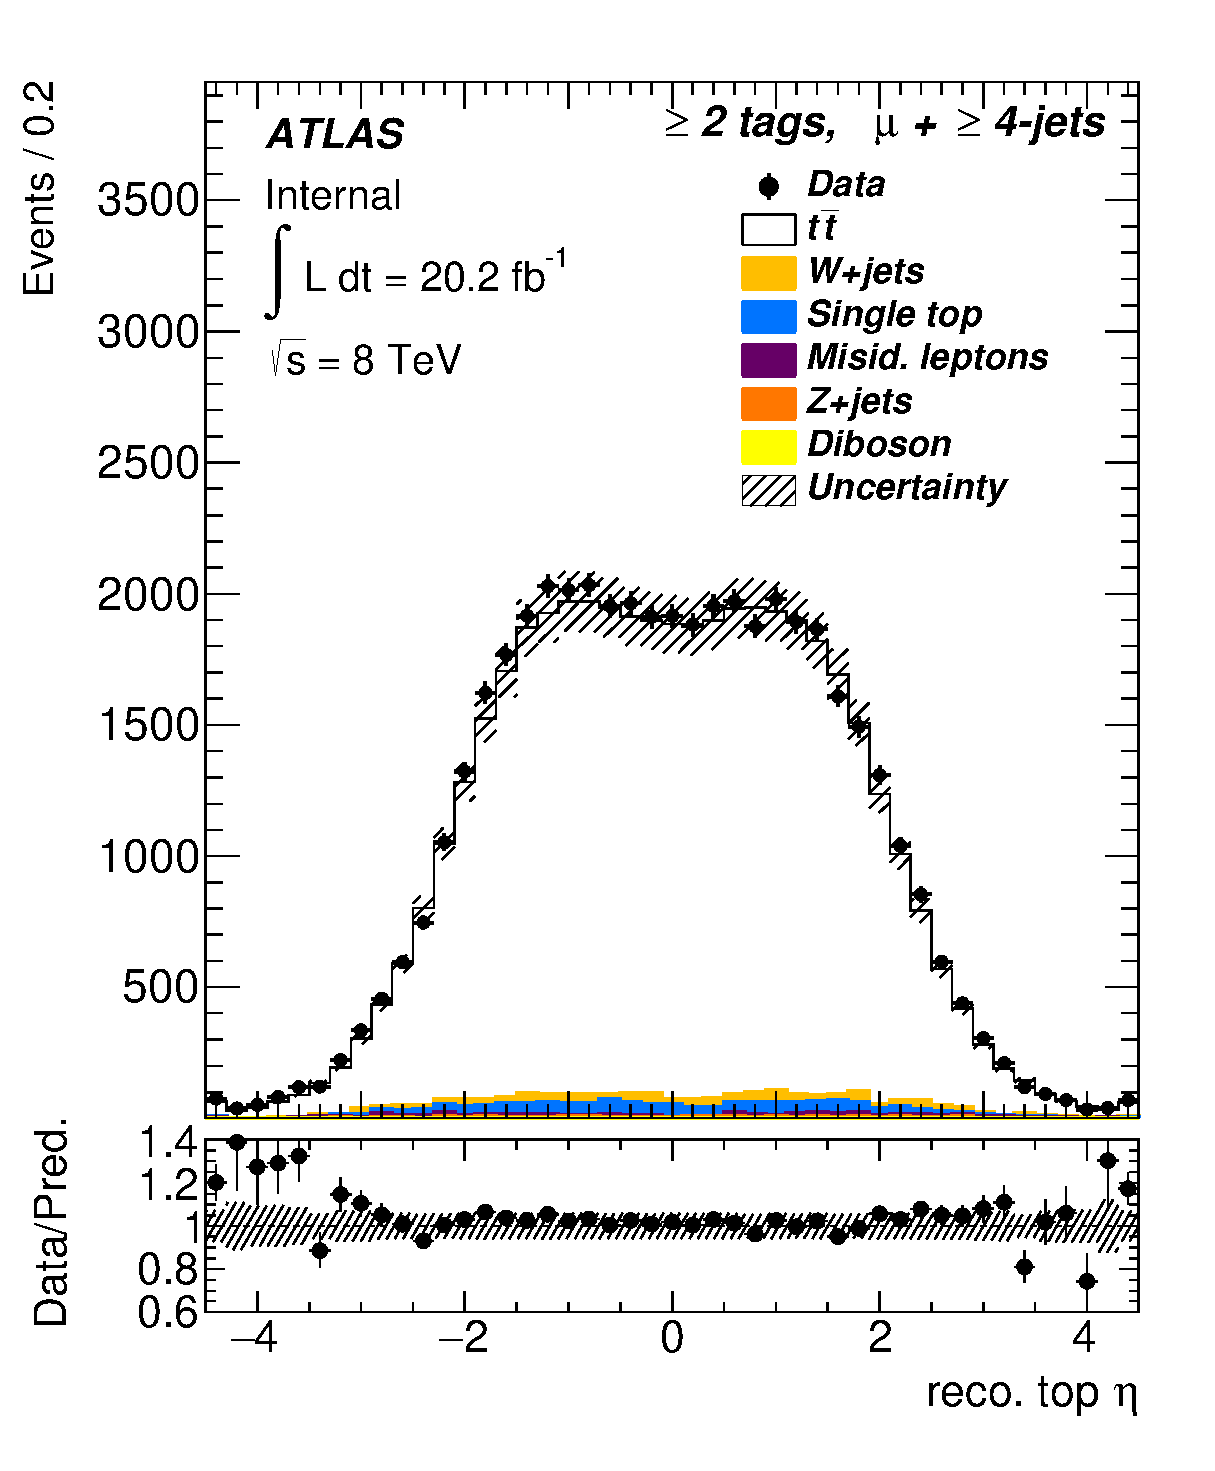
\includegraphics[height=65mm]{chapters/whel/figures/control_Plots2/bTag_2incl/reco_Top_eta_mu}\\
		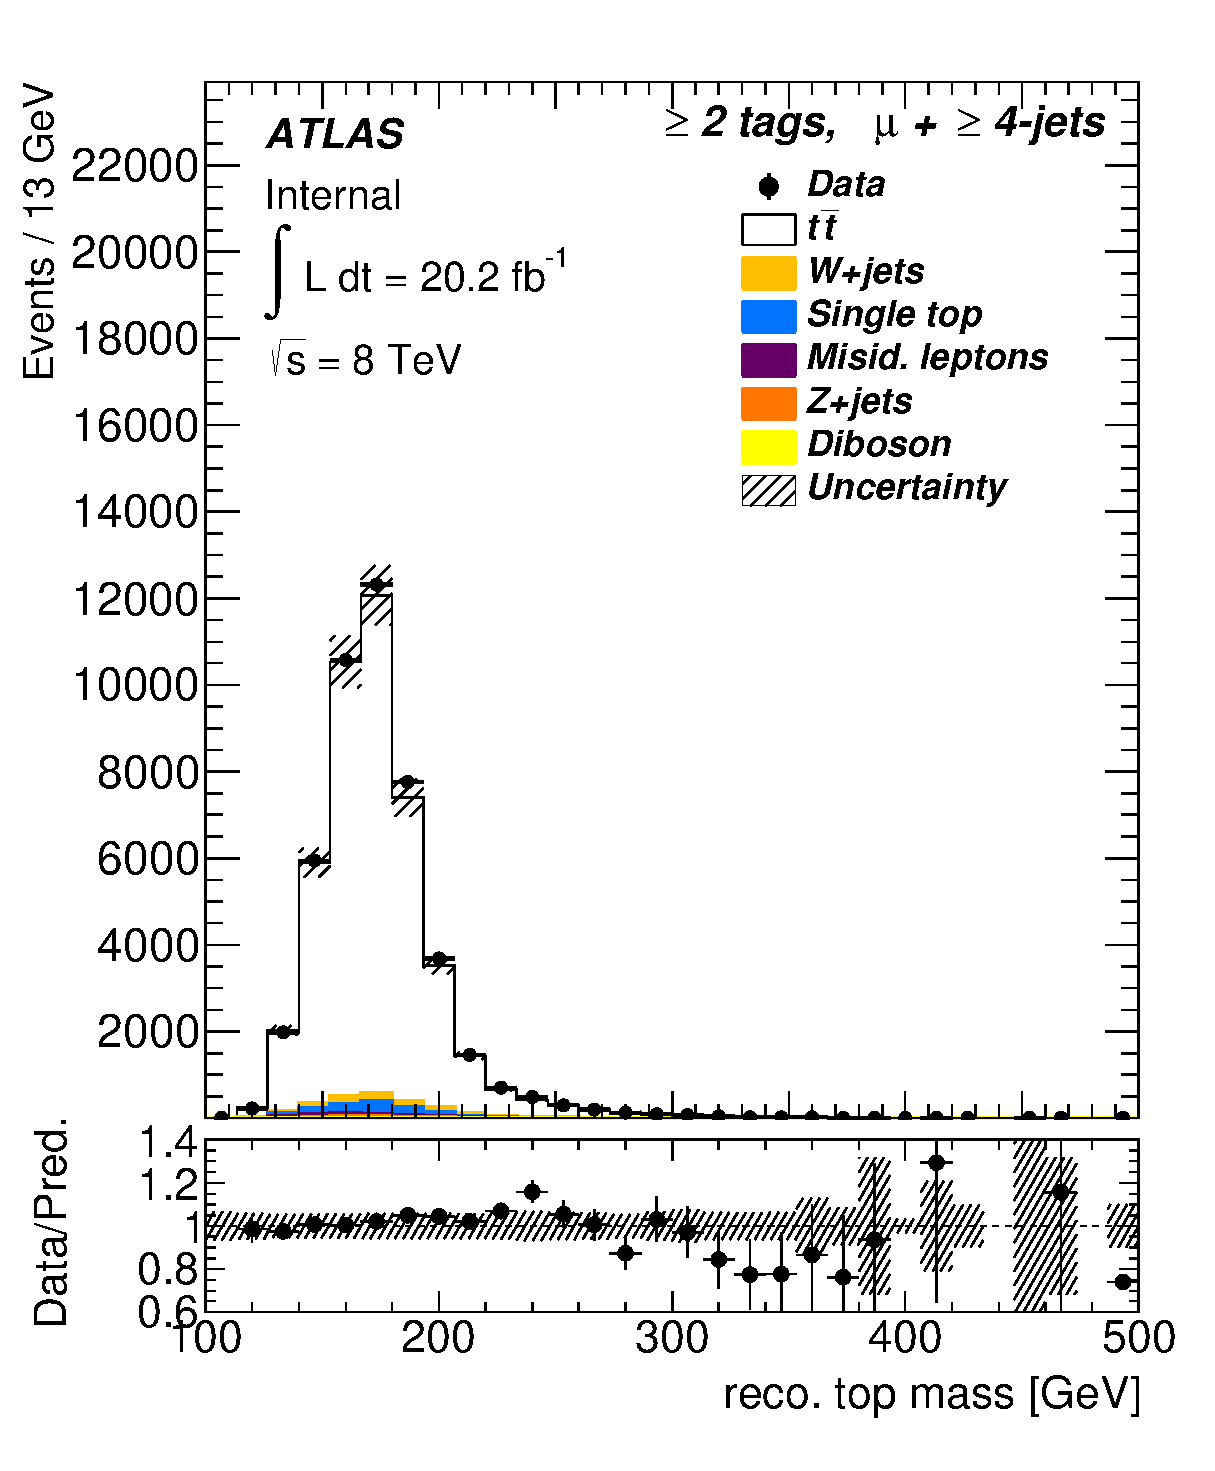
\includegraphics[height=65mm]{chapters/whel/figures/control_Plots2/bTag_2incl/reco_Top_m_mu}
		\includegraphics[height=65mm]{chapters/whel/figures/control_Plots2/bTag_2incl/NumberBtags_mu}\\
		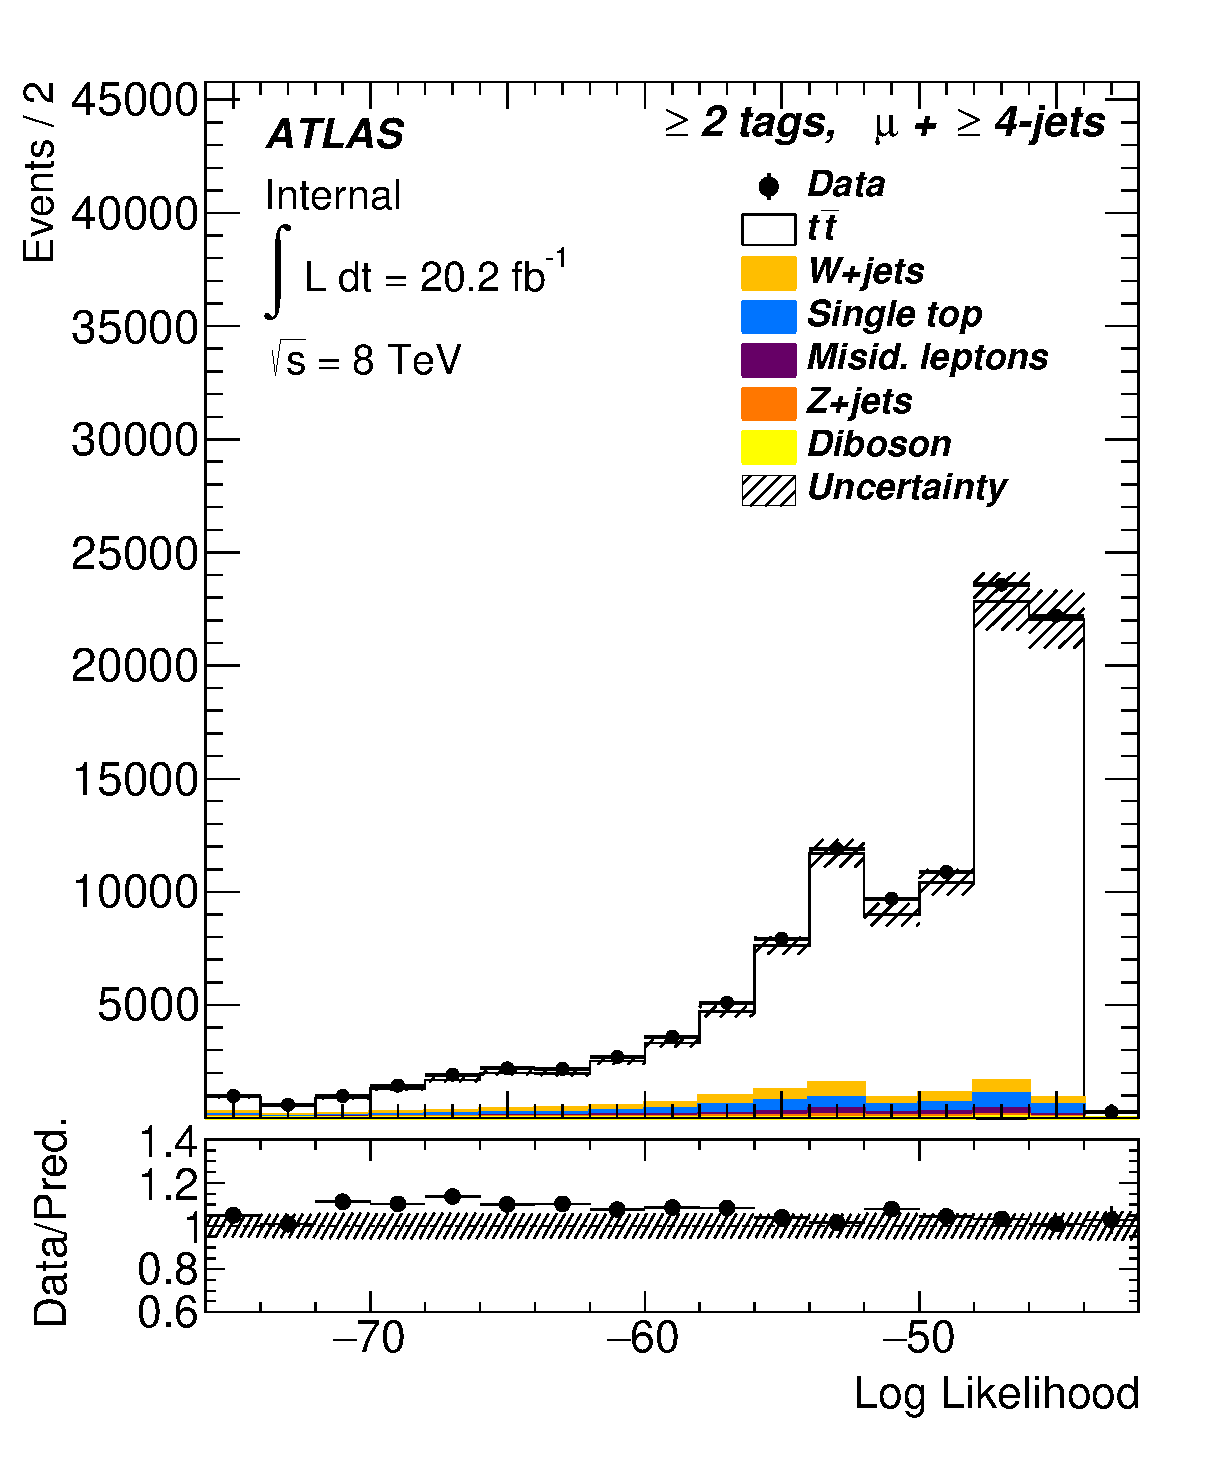
\includegraphics[height=65mm]{chapters/whel/figures/control_Plots2/bTag_2incl_NoLHCut/LogLikelihood_mu}
        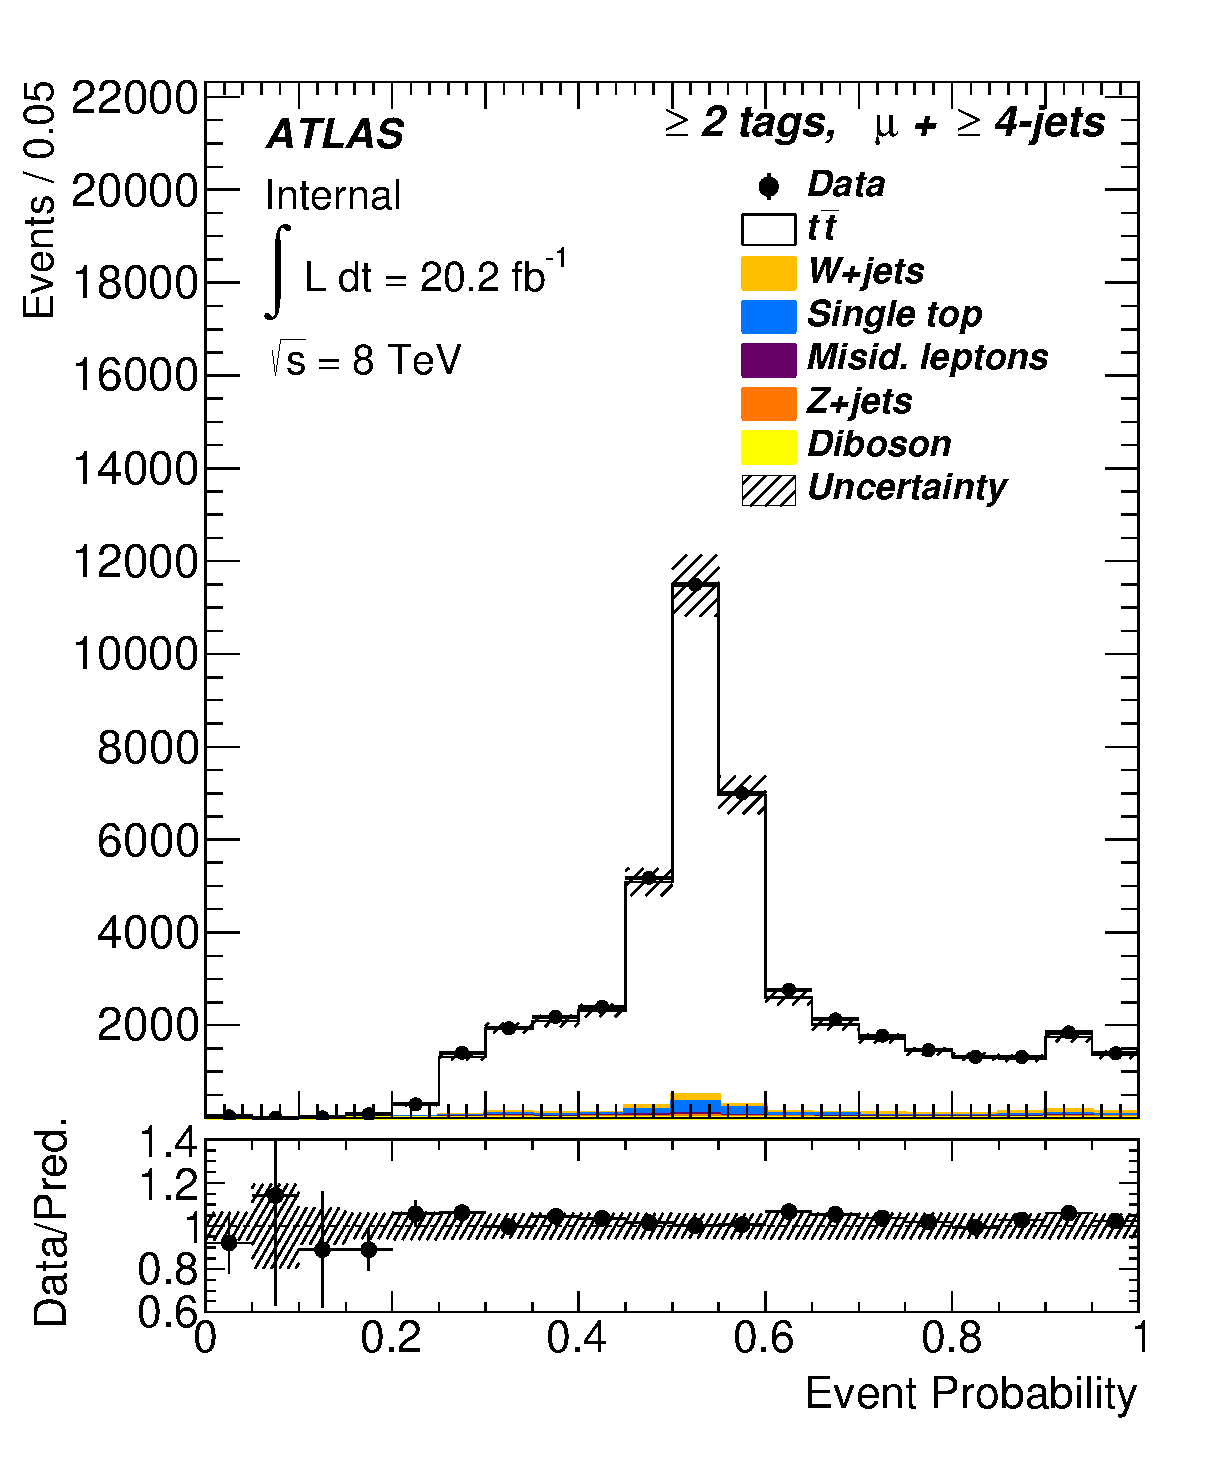
\includegraphics[height=65mm]{chapters/whel/figures/control_Plots2/bTag_2incl/EventProbability_mu}

	\caption{Control distributions in the 2 inclusive \bt tag, muon channel for selected top kinematics, the log likelihood, and the event probability distributions of the leading permutation (ranked by event probability). All plots except for the log likelihood are shown after the cut LH $> -48$. The shaded bands represent the Monte Carlo statistical uncertainties.}
	\label{fig:klfitter_control_plots_4}
	\end{center}    
	\end{figure}
%\clearpage
\subsection{Transfer Functions}
\label{sec:TF}
The transfer functions (TF) used in the kinematic fitter are derived for electrons, muons, light jets, \bt jets, and \met using the 8 TeV \ttbar MC sample described in Section \ref{sec:backgroundAndSignalModelling}. The difference between reconstructed energy and truth-level energy is fit using a double Gaussian functional form to determine the detector response for jets and electrons. A double Gaussian functional form was chosen in order to allow for the modeling of asymmetric tails in the detector response. The functional form of the transfer functions is given by
\begin{eqnarray}
W(\Delta E)=\frac{1}{\sqrt{2\pi}(p_2+p_3p_5)}\left[ e^{\frac{-(\Delta E-p_1)^2}{2p_2^2}}+p_3\cdot e^{\frac{-(\Delta E-p_4)^2}{2p_5^2}}\right]
\label{eq:TFeq}
\end{eqnarray}
where $\Delta E=\frac{E_{truth}-E_{reco}}{E_{truth}}$, and the parameters $p_i$ depend on the energy of the parton/lepton are parameterized depending on the parton/lepton type. As the best guess at leading order, a linear dependence is assumed. If another dependence is known by a physical motivation, the paramterization is adapted correspondingly. For example, in the case of jets and electrons, $p_2$ represents the calorimeter resolution and is hence parameterized as $\sim 1/\sqrt{E}$. If the linear assumption fails, it can also be replaced by heuristically determined parameterizations. In the case of electrons and jets, the parameterizations are 

\begin{eqnarray}
p_1=a_1+b_1\cdot E_{truth}\label{eq:TFp1}\\
p_2=a_2/\sqrt{E_{truth}}+b_2\label{eq:TFp2}\\
p_3=a_3+b_3\cdot E_{truth}\label{eq:TFp3}\\
p_4=a_4+b_4\cdot E_{truth}\label{eq:TFp4}\\
p_5=a_5+b_5\cdot E_{truth}\label{eq:TFp5}
\end{eqnarray}
The $a_i$'s and $b_i$'s are obtained from a global fit to each particle species and $\eta$ region. For muons, $E_{truth}$ is replaced with $p_{T}^{truth}$, and all $p_i$ are parameterized linearly, i.e. Equation~\ref{eq:TFp2} becomes $p_2=a_2+b_2\cdot E_{truth}$. 

Only reconstructed objects that are bi-uniquely (one and only one matching for both objects) matched to partons from the hard decay are used to derive the transfer functions. An object is considered matched if the $\Delta R$ between the reconstructed and truth object is less than 0.3. The matching efficiencies for jets are (unsurprisingly) dependent on the jets fed into the kinematic fitter, and these efficiencies are discussed further in Sec. \ref{sec:KLopt}.

As the detector response changes in different regions of the detector and for particles with different energy ranges, a number of transfer functions are defined for each particle species and binned in terms of $\eta$ and \pt.  %Fig X displays normalized transfer functions for a variety of particle species and \eta ranges.

\subsection{Hadronic Flavor Separation} 
\label{sec:udSep}
Directly extracting helicity fractions using the hadronic \w decay requires a correct reconstruction and identification of the flavor of the daughter jets. Since the \w and top masses for the hadronically decaying top are invariant under a permutation of the \w-daughter jets, a quantity including information beyond the kinematics is necessary to correctly assign the identities of all four jets in the hard \ttbar decay. This new quantity is called the event probability, and for a given permutation, $i$, is given by
\begin{eqnarray}
p_{i}= \frac{\mathcal{L}_i\prod_j\Delta p_{i,j}}{\sum_i\mathcal{L}_i\prod_j\Delta p_{i,j}}
\label{eq:probExt}
\end{eqnarray}
where the $\Delta p_{i,j}$'s are extensions or weights for each jet, $j$, in permutation $i$ which are convoluted with the likelihood in order to take advantage of information beyond the invariant masses of the candidate \w and top objects, e.g. the \bt tagging (MV1) weight of the jets. A simple extension using  \bt tagging information would be to apply a binary weight of 1(0) depending on whether a jet permuted into the position of a \bt jet has an MV1 weight larger(smaller) than a predefined threshold, e.g.
\begin{eqnarray}
\Delta p_{i,j}= %\left\{ \\FIXME?
\begin{array}{ll}
0 \text{  if jet position is for \bt jet and input jet is not \bt tagged}\\
1 \text{  if position is for \bt jet and input jet is \bt tagged}
%\right\} 
\end{array}
\label{eq:bTag_pij}
\end{eqnarray}


To extract the helicity fractions in the hadronic channel, an extension must be defined that takes advantage of information that can distinguish between the up and down type jets of the \w decay. The \pt of the light jets can be used to separate up-type from down-type jets since the $V-A$ structure of the \Wtb vertex predicts an imbalance in their energies \cite{Jezabek:1994zv,Brandenburg:2002xr}. This difference is the most pronounced in the top rest-frame, but differences between the measured jet \ensuremath{p_{\text{T}}}'s are also observable in the lab-frame and are simpler to use. The jet \pt shapes for different flavor types are shown in Figure \ref{fig:udSeparation_templates}, but the separation power from this effect alone is quite small. 

The MV1 weights of the two light jets are also be used to discriminate between up and down type jets. Compared to jets coming from $u,d,$ and $s$ quarks, jets coming from $c$ quarks have, on average, considerably higher MV1 weights. This discrimination is observable in Figure \ref{fig:udSeparation_templates}. \Wboson bosons decaying via $W\rightarrow c\bar{s}$ (about 50\,\% of all hadronically decaying \Wboson bosons) allow the MV1 information to help identify light jet flavors in a large number of reconstructed events. 

\begin{figure}[!ht]
  %\begin{center}
    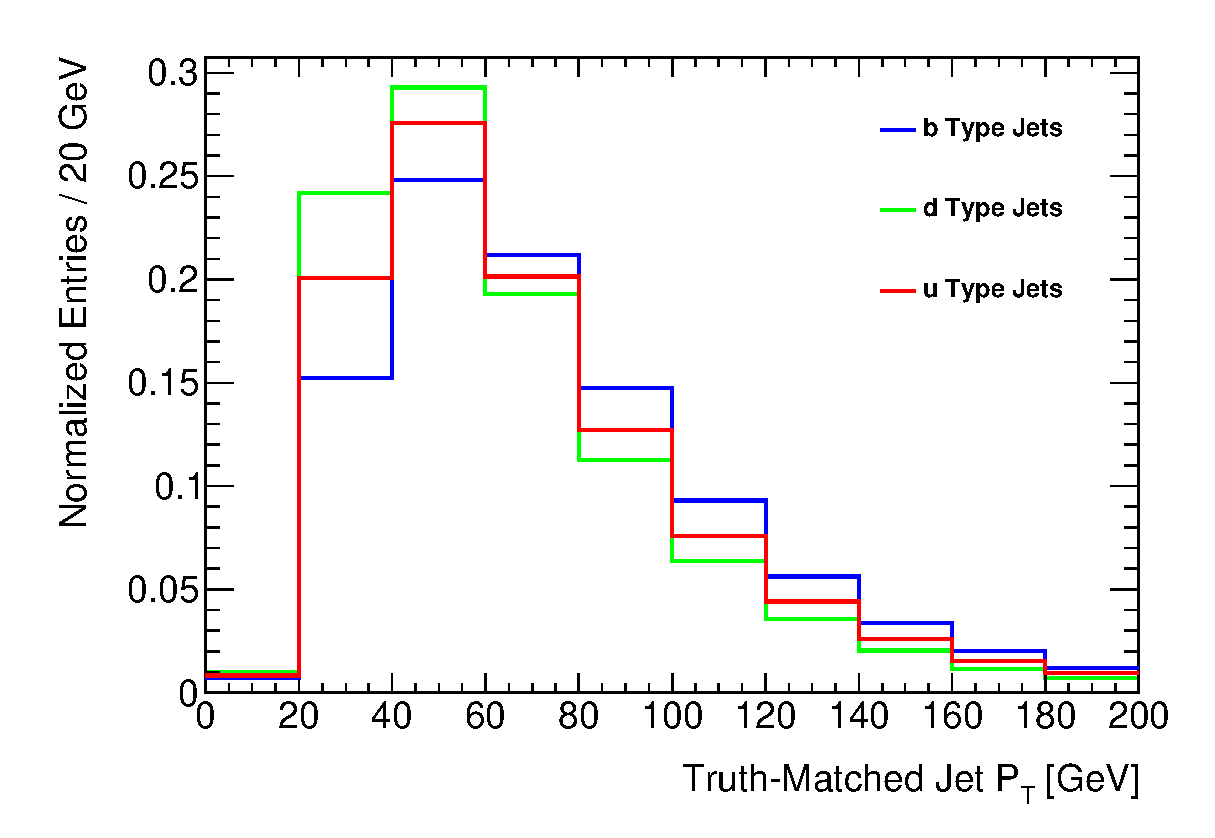
\includegraphics[height=50mm]{chapters/whel/figures/pt_template_5jetOPT}
    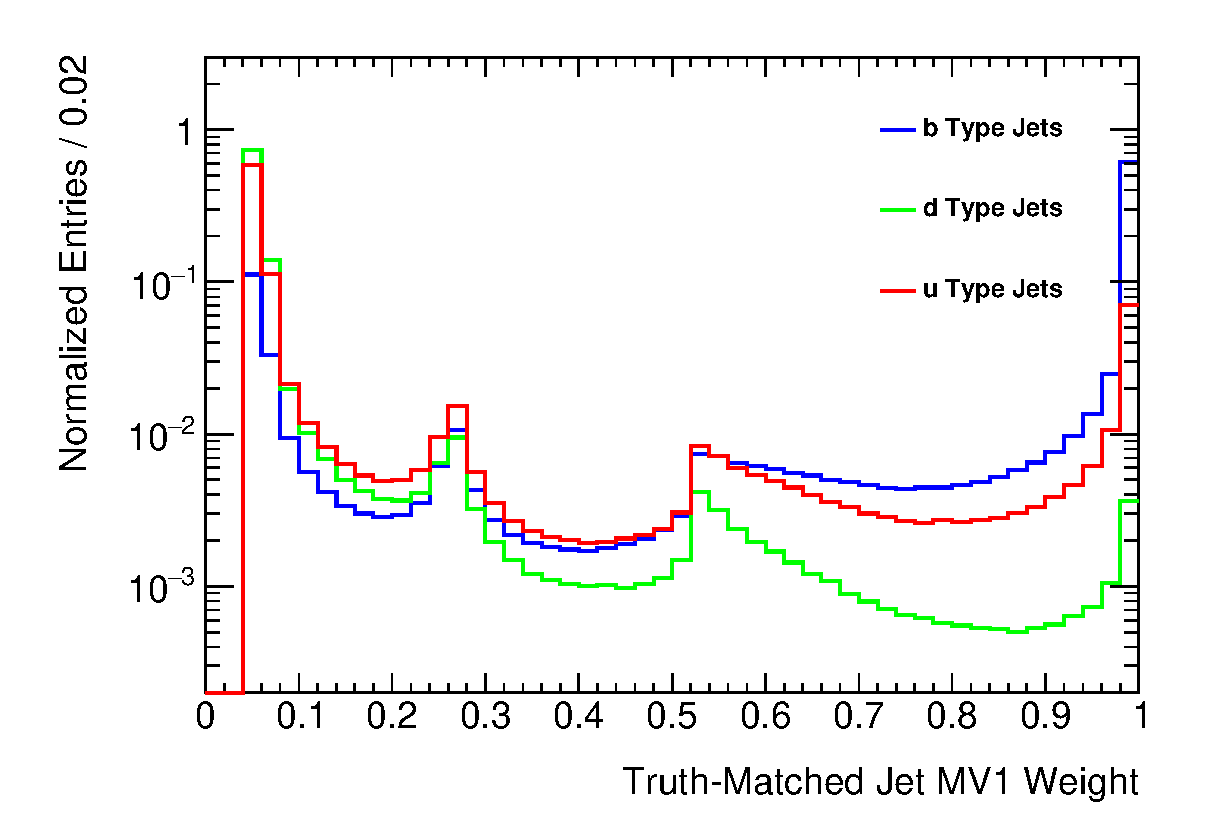
\includegraphics[height=50mm]{chapters/whel/figures/mv1_template_5jetOPT}
    \caption{Templates of reconstructed \pt and MV1 weight for truth-matched u-type, d-type, and \bt jets. These templates are used as inputs to the u/d separation configuration of KLFitter.}
    \label{fig:udSeparation_templates}
  %\end{center}
\end{figure}

Using both of these variables, an extension for separating up and down type jets (`u/d separation') can be calculated using templates of the reconstructed jet \pt and MV1 distributions. This approach follows the path taken by the 7 TeV ATLAS measurement of spin correlation in semileptonic \ttbar events \cite{7tev_spin_ljets}. The templates were created for up-type ($q=u,c$), down-type ($q=d,s$), and \bt jets ($q=b$) using the 8 TeV \ttbar Monte Carlo signal sample. The reconstructed jets must be bi-uniquely matched ($\Delta R \leq 0.3$) to one of the quarks produced in the \ttbar decay in order to counted in the templates. Using these templates, the product of the probability extensions for all jets in one fit is formally given as 
\begin{eqnarray}
\Delta p_{i, \text{u/d sep}}= 
\text{P}^{\text{ b-type}}(\pt^{\text{ blep}})\cdot 
\text{P}^{\text{ b-type}}(MV1^{\text{ blep}})\cdot 
\text{P}^{\text{ b-type}}(\pt^{\text{ bhad}})\cdot
\text{P}^{\text{ b-type}}(MV1^{\text{ bhad}})\cdot\\
\text{P}^{\text{ u-type}}(\pt^{\text{ u-jet}})\cdot 
\text{P}^{\text{ u-type}}(MV1^{\text{ u-jet}})\cdot 
\text{P}^{\text{ d-type}}(\pt^{\text{ d-jet}})\cdot
\text{P}^{\text{ d-type}}(MV1^{\text{ d-jet}})
\label{eq:ud_pij}
\end{eqnarray}
where $P()$'s represent the probability of a particular jet to have its measured values of \pt and MV1 given the jet assignment (\bt from leptonic top (blep), \bt from hadronic top (bhad), u-jet, d-jet) in the current permutation. The individual jet weights are calculated using the templates in Figure \ref{fig:udSeparation_templates} normalized to unity. Using these weights, the event probability is calculated for each permutation. The permutation with the highest event probability is then chosen as the final permutation for the extraction of the helicity angles for both \w's from the \ttbar decay. Dedicated linearity tests were performed to check whether the use of templates based on the \pt of the jets introduces a bias for left-handed events. %The calibration curves resulting from the lineary tests can be found in Appendix~\ref{app:fitCalibrations}. 
The hadronic linearity tests were found to perform well under closure, and no bias was observed.

\subsection{KLFitter Optimization Study}
\label{sec:KLopt}
The efficiency of the kinematic fitting to correctly identify jet assignments relies on the jets available for permutation. Since each position is unique in the u/d separation configuration (even though swapping the positions of the light jets from \w decay is invariant under the \w mass constraint), supplying KLFitter with $n$ jets requires the likelihood calculation for $n!$ permutations. The optimal jet input configuration should maximize the matching efficiency of the reconstruction while balancing the CPU time required for each event. %Given the factorial increase in computing time, KLFitter itself is limited to accepting no more than 5 jets. 
The matching efficiency is defined as
\begin{eqnarray}
\upepsilon_{\text{match}}=N_{\text{events}}^{\text{match}}/N_{\text{events}}^{\text{total}}
\label{eq:matchEff}
\end{eqnarray}
where $N_{\text{events}}^{\text{match}}$ can be defined in many ways (e.g. correctly matching all four jets, correctly matching only the three jets necessary for the hadronic angle, correctly matching only the \bt jets, etc.). In the following discussion, an event is considered matched for the leptonic angle when both \bt jets be correctly matched while all four jets are required to be correctly matched in in the hadronic case. Using these definitions, the final matching efficiencies are computed for both channels to find the optimal jet input configuration.

Many previous ATLAS \ttbar analyses use the four leading jets in \pt as input to reconstruct the \ttbar system. The simplest extension is increasing the number of input jets to five. In this case, the fitter will iterate through $5!=120$ permutations. Another option is to change the ordering by which jets are chosen to be included in the fit. In the 8 TeV ATLAS measurement of \ttbar charge asymmetry \cite{Juste:1647184}, the two jets (taken from all jets passing object selection in the event) with the highest MV1 weights are selected, and then the remaining jets are re-ordered in \pt and the three highest taken as input. 

For this analysis, three different input configurations were studied: four leading jets in \pt (4-jet simple), five leading jets in \pt (5-jet simple), two leading jets in MV1 + three highest \pt jets remaining (5-jet advanced). The results are presented in Table \ref{tab:matchEff}.

\begin{table}[]
\centering
\begin{tabular}{l|l}
\hline \hline
Configuration  & $\ell$+jets \\ \hline
4-jet simple     &  0.260   \\
5-jet simple     &  0.292   \\
5-jet advanced   &  0.323   \\ \hline \hline
\end{tabular}
\caption{Matching efficiencies for different KLFitter input jet configurations. An event is considered matched if all four truth jets from the hard \ttbar decay are bi-uniquely matched (within a $\Delta R\leq 0.3$) to four reconstructed jets of the leading KLFitter permutation.}
\label{tab:matchEff}
\end{table}

Since the 5-jet advanced configuration was found to have the highest efficiency and the computing time required was reasonable, it was chosen as the final configuration for the extraction of the helicity fractions in both the leptonic and hadronic channels.

\subsection{Optimizing hadronic sensitivity}
\label{sec:hadronicOptimization}
Helicity fractions extracted from the hadronic \w decay are less sensitive than the corresponding fractions extracted from the leptonic \w decay since the daughter down-type jet is, in general, harder to correctly identify than a charged lepton (electron or muon). If the u/d separation procedure detailed in Section \ref{sec:udSep} were 100\% efficient, the pure helicity templates for the hadronic decay (Figure~\ref{fig:Sig_temp_had}) would be expected to follow the theoretical curves for pure helicity states as in the case of the leptonic templates (Figure~\ref{fig:Sig_temp_lep}). Incorrectly assigned jets (and swapping between the two hadronic W daughters) lead to left-handed and right-handed templates that closely resemble one another other. 

Selecting a subset of reconstructed events which contain a relatively higher fraction of correctly matched events should provide a larger separation between hadronic signal templates and lead to a more sensitive result. To this end, four categories of \ttbar reconstruction are defined, and the resulting categories plotted to identify regions with higher proportions of correctly matched events:

\begin{itemize}
\item \textbf{Right}: All 4 jets uniquely truth-matchable, fed into KLFitter, and correctly assigned in the leading permutation
\item \textbf{Wrong}: All 4 jets uniquely truth-matchable, fed into KLFitter, but not correctly assigned in the leading permutation
\item \textbf{Non-reco}: Due to acceptance loss or non-unique matching, not all four jets from the hard \ttbar decay can  be matched to reconstructed objects
\item \textbf{Bkg}: Dileptonic or tauonic \ttbar decays where no true hadronic angle exists
\end{itemize}

In Figure \ref{fig:hadronicOpt_stack}, the \ttbar distributions for the event probability and log likelihood are broken into the above categories and shown for the leading KLFitter permutation in the electron channel. Both plots are normalized to the total \ttbar yield from the 2012 dataset.

\begin{figure}[htbp]
\begin{center}
		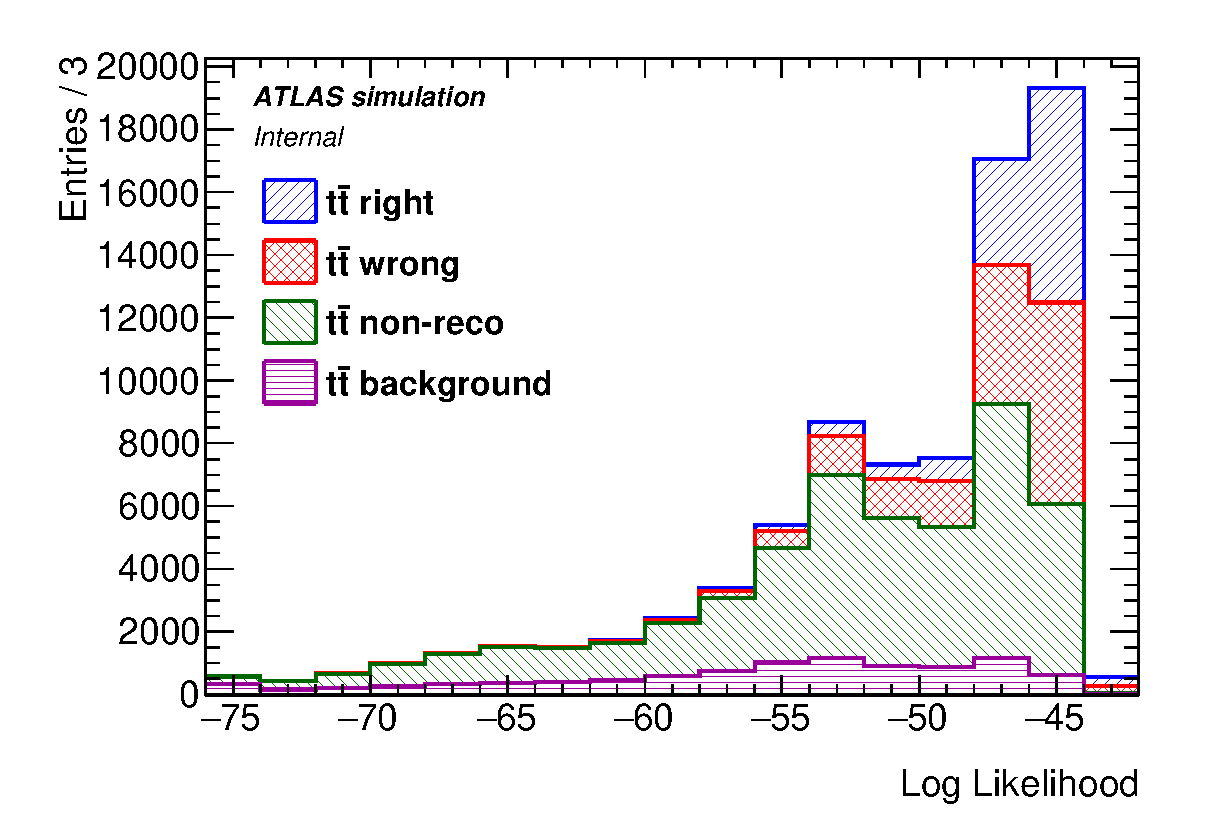
\includegraphics[height=50mm]{chapters/whel/figures/lh_stack}
		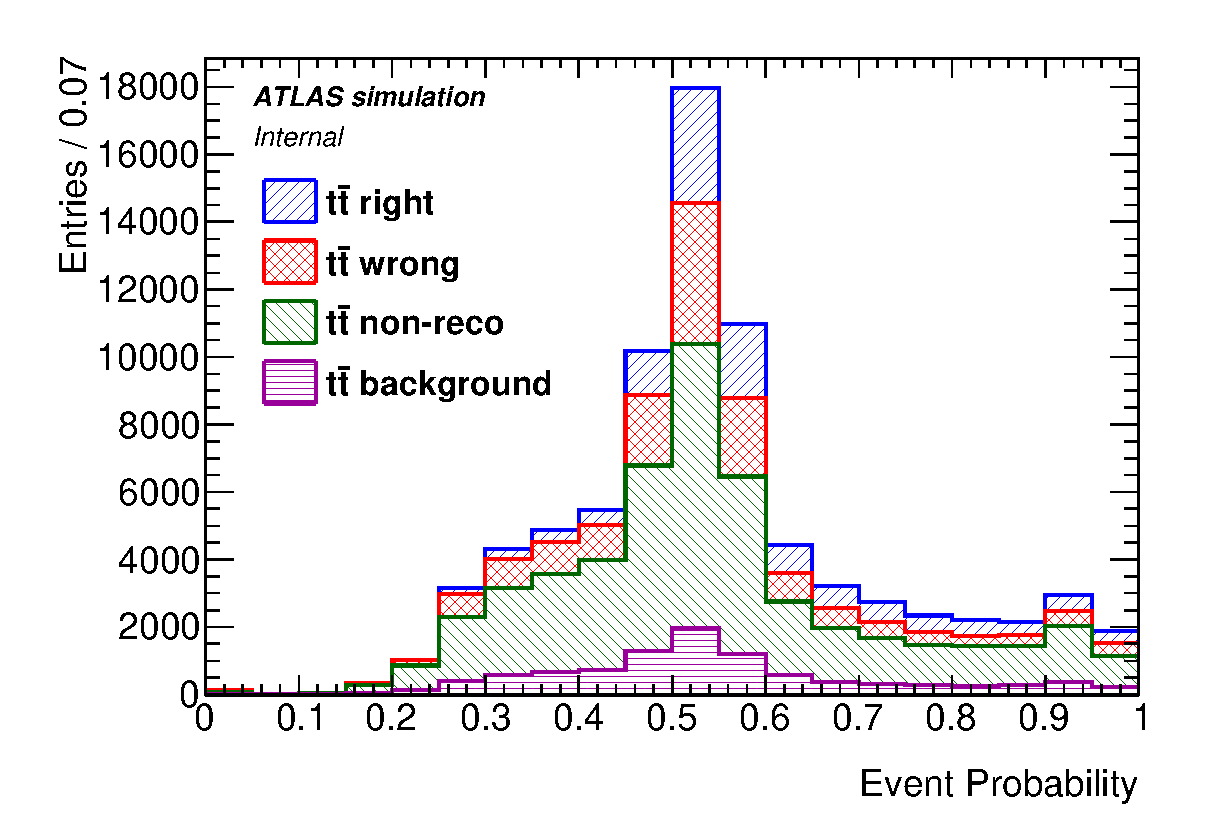
\includegraphics[height=50mm]{chapters/whel/figures/evProb_stack}
		\caption{Categorized \ttbar distributions for log likelihood and event probability of leading KLFitter permutation. Total yield is normalized to \ttbar yield from 20.3 fb$^{-1}$.}
	\label{fig:hadronicOpt_stack}
\end{center}	
\end{figure}

While there is no region with clear concentration of correctly matched \ttbar in the event probability distribution, correct matched events are concentrated in the log likelihood distribution above values of -55.

To optimize the statistical sensitivity of the hadronic templates, several fits in the two inclusive \bt tag region were performed scanning across a number of cuts on the log likelihood of the best permutation. The template fitting method used to study the effect of the likelihood cuts on the statistical sensitivity is discussed in Section \ref{sec:templateFitting}. The background normalizations in the fit were kept fixed in order to isolate the effect of the likelihood cut on the \ttbar signal. Results of the sensitivity on the extracted fractions and the signal efficiencies as a function of the likelihood cut are shown in Table \ref{tab:hadOpt_table}.

\begin{table}[h!]
\centering
    \begin{tabular}{c | c | c | c | c}
        Channel & LH $>-49$ & LH $>-48$ & LH $>-47$ & LH $>-46$\\
        \hline
         \hfill$\sigma_{F_0}$                    &  0.0168$\pm$0.0002  &  0.0167$\pm$0.0002  &  0.0174$\pm$0.0002  &  0.0193$\pm$0.0002 \\
        \textbf{$e$+jets} \hfill$\sigma_{F_L}$   &  0.0299$\pm$0.0003  &  0.0301$\pm$0.0003  &  0.0299$\pm$0.0003  &  0.0350$\pm$0.0003 \\
         \hfill$\sigma_{F_R}$                    &  0.0293$\pm$0.0003  &  0.0285$\pm$0.0003  &  0.0288$\pm$0.0003  &  0.0324$\pm$0.0003 \\
        \hline
         \hfill$\sigma_{F_0}$                    &  0.0159$\pm$0.0002  &  0.0161$\pm$0.0002  &  0.0170$\pm$0.0002  &  0.0193$\pm$0.0002 \\
        \textbf{$\mu$+jets}\hfill$\sigma_{F_L}$  &  0.0285$\pm$0.0003  &  0.0281$\pm$0.0003  &  0.0297$\pm$0.0003  &  0.0353$\pm$0.0004 \\
         \hfill$\sigma_{F_R}$                    &  0.0273$\pm$0.0003  &  0.0268$\pm$0.0003  &  0.0288$\pm$0.0003  &  0.0337$\pm$0.0004 \\\hline
         \multicolumn{5}{c}{ }\\
         \hline
         LH Cut Efficiency &  0.418 &  0.375  &  0.308  &  0.212 \\
        \hline
      \end{tabular}
      \caption{Top: scan of log likelihood cuts designed to find value that yields optimal statistical sensitivity of hadronic helicity fraction extraction. A log likelihood cut of $>$ -48 was found to have the best sensitivity. Bottom: \ttbar efficiency for each likelihood cut in the scan.}
    \label{tab:hadOpt_table}
    \end{table}

A log likelihood cut of $>-48$ is found to optimize the statistical sensitivity in the hadronic channel. An identical study on the leptonic angle showed no significant gain (or loss) in sensitivity for any cut on likelihood, so the hadronically optimal cut of log likelihood $> -48$ was applied to all events for both angles to simplify combinations between the leptonic and hadronic channels. Plots for both lepton channels and \bt tag regions showing data/prediction comparisons after event reconstruction and the log likelihood cut are shown in Figures \ref{fig:control_plots_el_1excl}-\ref{fig:control_plots_mu_2incl}. The log likelihood plots are shown before the likelihood cut is applied.


%------------------------------------------------------------------------------Gvantsa
%\subsection{Dilepton Channel} 
%Reconstructing the \ttbar kinematics in the dilepton channel is challenging due to the
%two neutrinos in the final state, making the system underconstrained.  Hence, assumptions are mandatory to perform the \ttbar reconstruction in this channel in order to measure the W helicity fractions.  Several methods have been used previously in different measurements at the LHC and Tevatron to reconstruct the \ttbar kinematics in the dilepton channel. In this analysis is used Kinematic method (KIN) [Phys. Rev. D73:112006, 2006.,Phys.Lett., B722:48–54, 2013.]. 
%\subsubsection{Kinematic method} 
%Assuming the process $pp -> \ttbar +X ->W^+bW^-\bbar+X->l^+\bar\nu b l^- \bar{\nu} \bbar+X $, the following kinematic constraints can be set:

%\begin{center} $p_b+p_{W^+}=p_t$, \newline
%$p_{\bbar}+p_{W^-}=p_{\tbar}$,\newline
%$p_{l^+}+p_{\nu}=p_{W^+}$,\newline
%$p_{l^-}+p_{ \bar{\nu} }=p_{W^-}$,\newline
%$p_{\nu_x}+p_{ \bar{\nu}_x }=E_x^{miss}$,\newline
%$p_{\nu_y}+p_{ \bar{\nu}_y }=E_y^{miss}$.\newline
%\end{center}
%Asuumptions: $m_W =80.4$ \gev and $m_{\nu} =0.$ \gev. The above set of equations has one less constraints than the number of measured variables.  In order to solve this underconstrained system,
%certain assumptions have to be made. For instance, by specifying a value for the top quark mass, this set of equations can be solved and the four vectors of $t$ and$\tbar$ will be determined.
%There are two types of ambiguities  which still need to be resolved. First,  the set of equations  is
%equivalent to a polynomial of the 4-th order in one selected variable.  Therefore, there can be up to four real solutions.  Second, even in the simplest case of two leptons and just two jets in the final state, there is a twofold ambiguity to assign the lepton and b-jet to the proper top quark.  Furthermore, one has to address the possibility of having more than two jets in the final state which increases this ambiguity even more.  Finally, one also needs to address the fact that the measured quantities entering the equations are subject to experimental uncertainties.
%------------------------------------------------------------------------------Gvantsa
\clearpage
